\section{Anwendungsschicht}
	Netzwerkanwendung: \newline
	\begin{itemize}
  	\item Anwendungsprozesse auf verschiedenen Hosts
  	\item kann direkt unter Verwendung der Dienste der Transportschicht implementiert werden
	  \item standardisieret Anwendung benutzen ein Anwendungsprotokoll, das das Format der Nachrichten und das Verhalten beim Empfang festlegt
	\end{itemize}
	\subsection{Paradigmen}
		\subsubsection{Client-Server}
			Server stellt Dienst zur Verfügung, der vom Client angefragt wird
		\subsubsection{Wechselnde Rollen}
			Hosts übernehmen mal die eine, mal die andere Rolle
		\subsubsection{Verteilte Anwendung}
			Besteht aus mehreren unabhängigen Anwendungen, die zusammen wie eine einzelne Anwendung erscheinen (z.B. WebShop mit Web-Server, Applikations-Server und Datenbank), Koordination ist zwar verteilt, findet aber für das Gesamtsystem statt
		\subsubsection{Peer-to-Peer}
			Vernetzung von Gleichen: \newline
			\begin{itemize}
				\item dezentrale Architektur (z.B. Bitcoin)
				\item Hybridarchitektur: Initialisierung findet über zentrale Architektur statt, Anwendung dezentral zwischen Hosts
			\end{itemize}
		\subsubsection{Anforderungen}
			\begin{itemize}
				\item Verlust
				\item Bitrate
				\item Verzögerungszeit
			\end{itemize}
	\subsection{Hypertext Transfere Protocol (HTTP)}
		\subsubsection{Ablauf}
			\begin{enumerate}
				\item Benutzer gibt URI (Uniform Resource Identifier) in Web-Browser ein
				\item URI enthält Host-Namen eines Web-Servers und den Pfad zu einem Objekt
				\item Web-Browser stellt Anfrage an Web-Server für dieses Objekt
				\item Web-Server liefert Objekt an Web-Browser zurück
				\item Web-Browser stellt Objekt für Nutzer lesbar da
			\end{enumerate}
		\subsubsection{Format der Anfragen}
			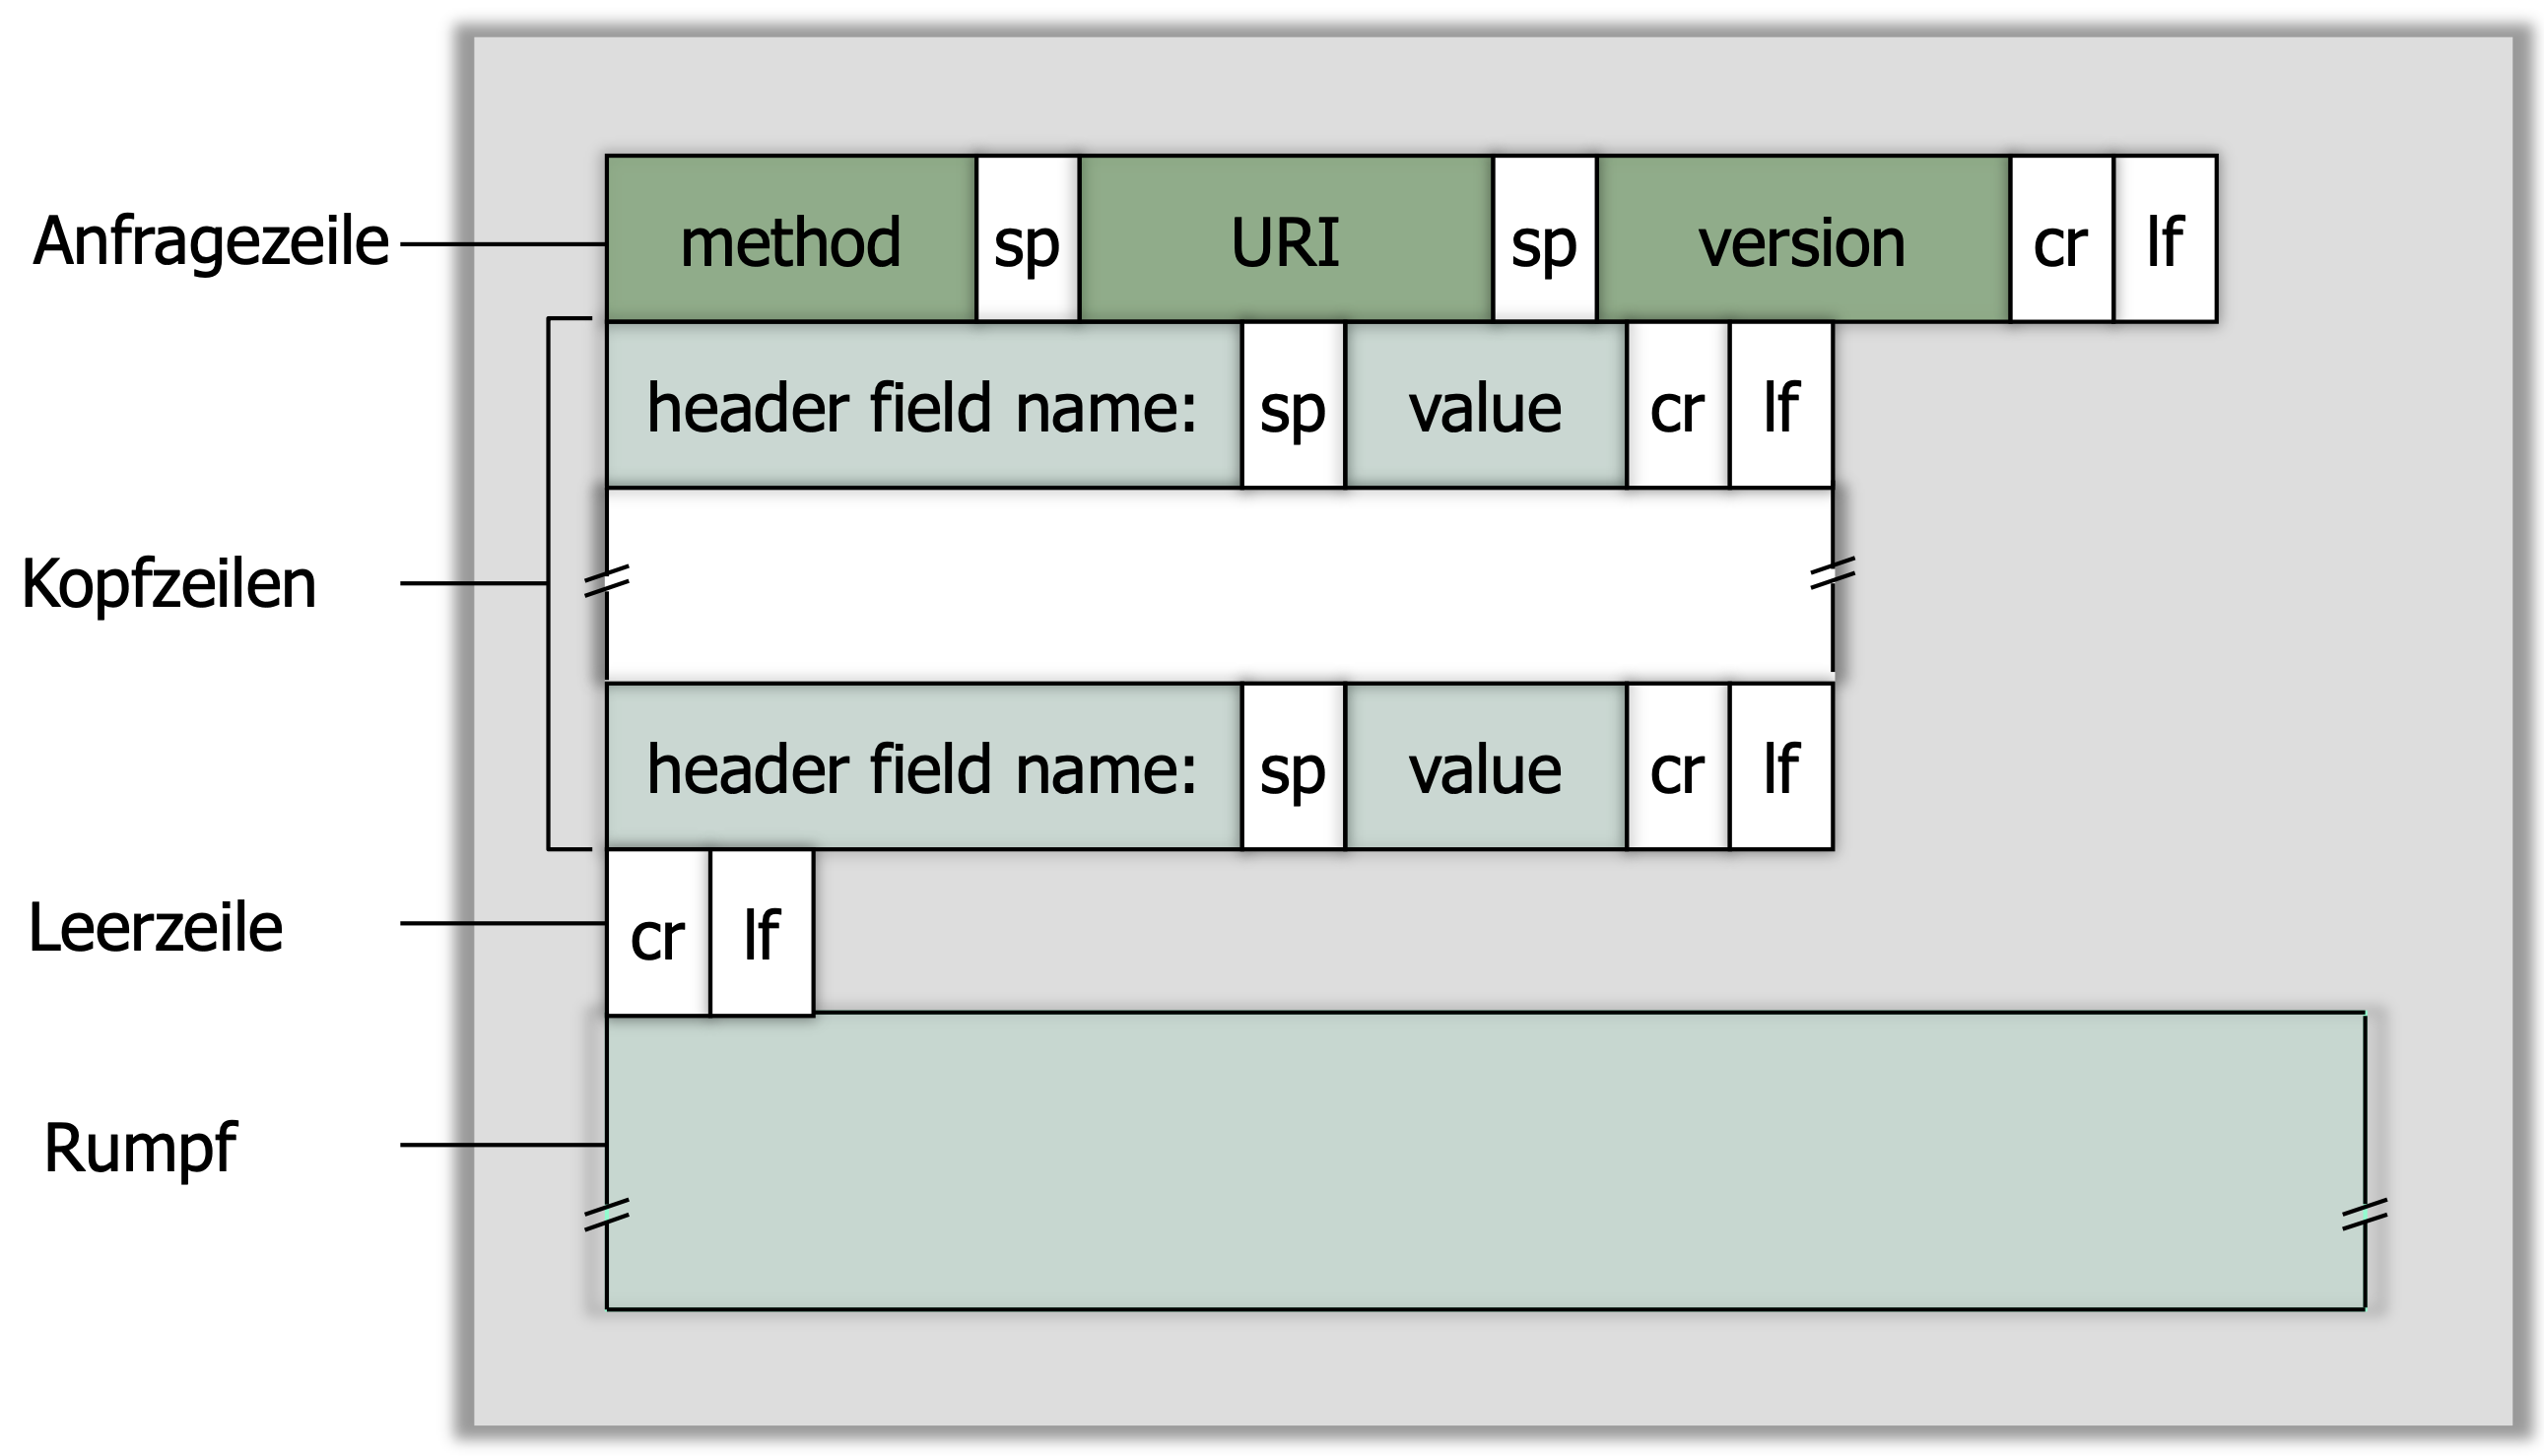
\includegraphics[scale=0.25]{Anfragenachricht_HTTP.png}
			\captionof{figure}{Anfrage}
		\subsubsection{Anfragenachricht}
			\begin{itemize}
				\item Methoden: 
					\begin{itemize}
						\item GET: Abruf eines Dokuments, besteht aus Methode, URI, Version
						\item HEAD: Abruf von Metainformationen eines Dokuments
						\item POST: Übergabe von Informationen an Server
						\item PUT
						\item DELET
					\end{itemize}
				\item Kopfzeilen:
					\begin{itemize}
						\item Typ/Wert-Paare, Typen: Host, User-agent, ...
					\end{itemize}
				\item Rumpf:
					\begin{itemize}
						\item leer bei GET, kann bei POST Inhalt haben
					\end{itemize}
			\end{itemize}
			\begin{center}
				\begin{tabular}{|cc|}
					\hline
					GET: & /somedir/page.html HTTP/1.1 \\
					HOST: & www.someschool.edu \\
					User-agent: & Mozilla/4.0 \\
					Connection: & close \\
					Accept-language: & de-de \\
					\hline
				\end{tabular}
				\captionof{figure}{Anfragenachricht}
			\end{center}
		\subsubsection{Format der Antworten}
			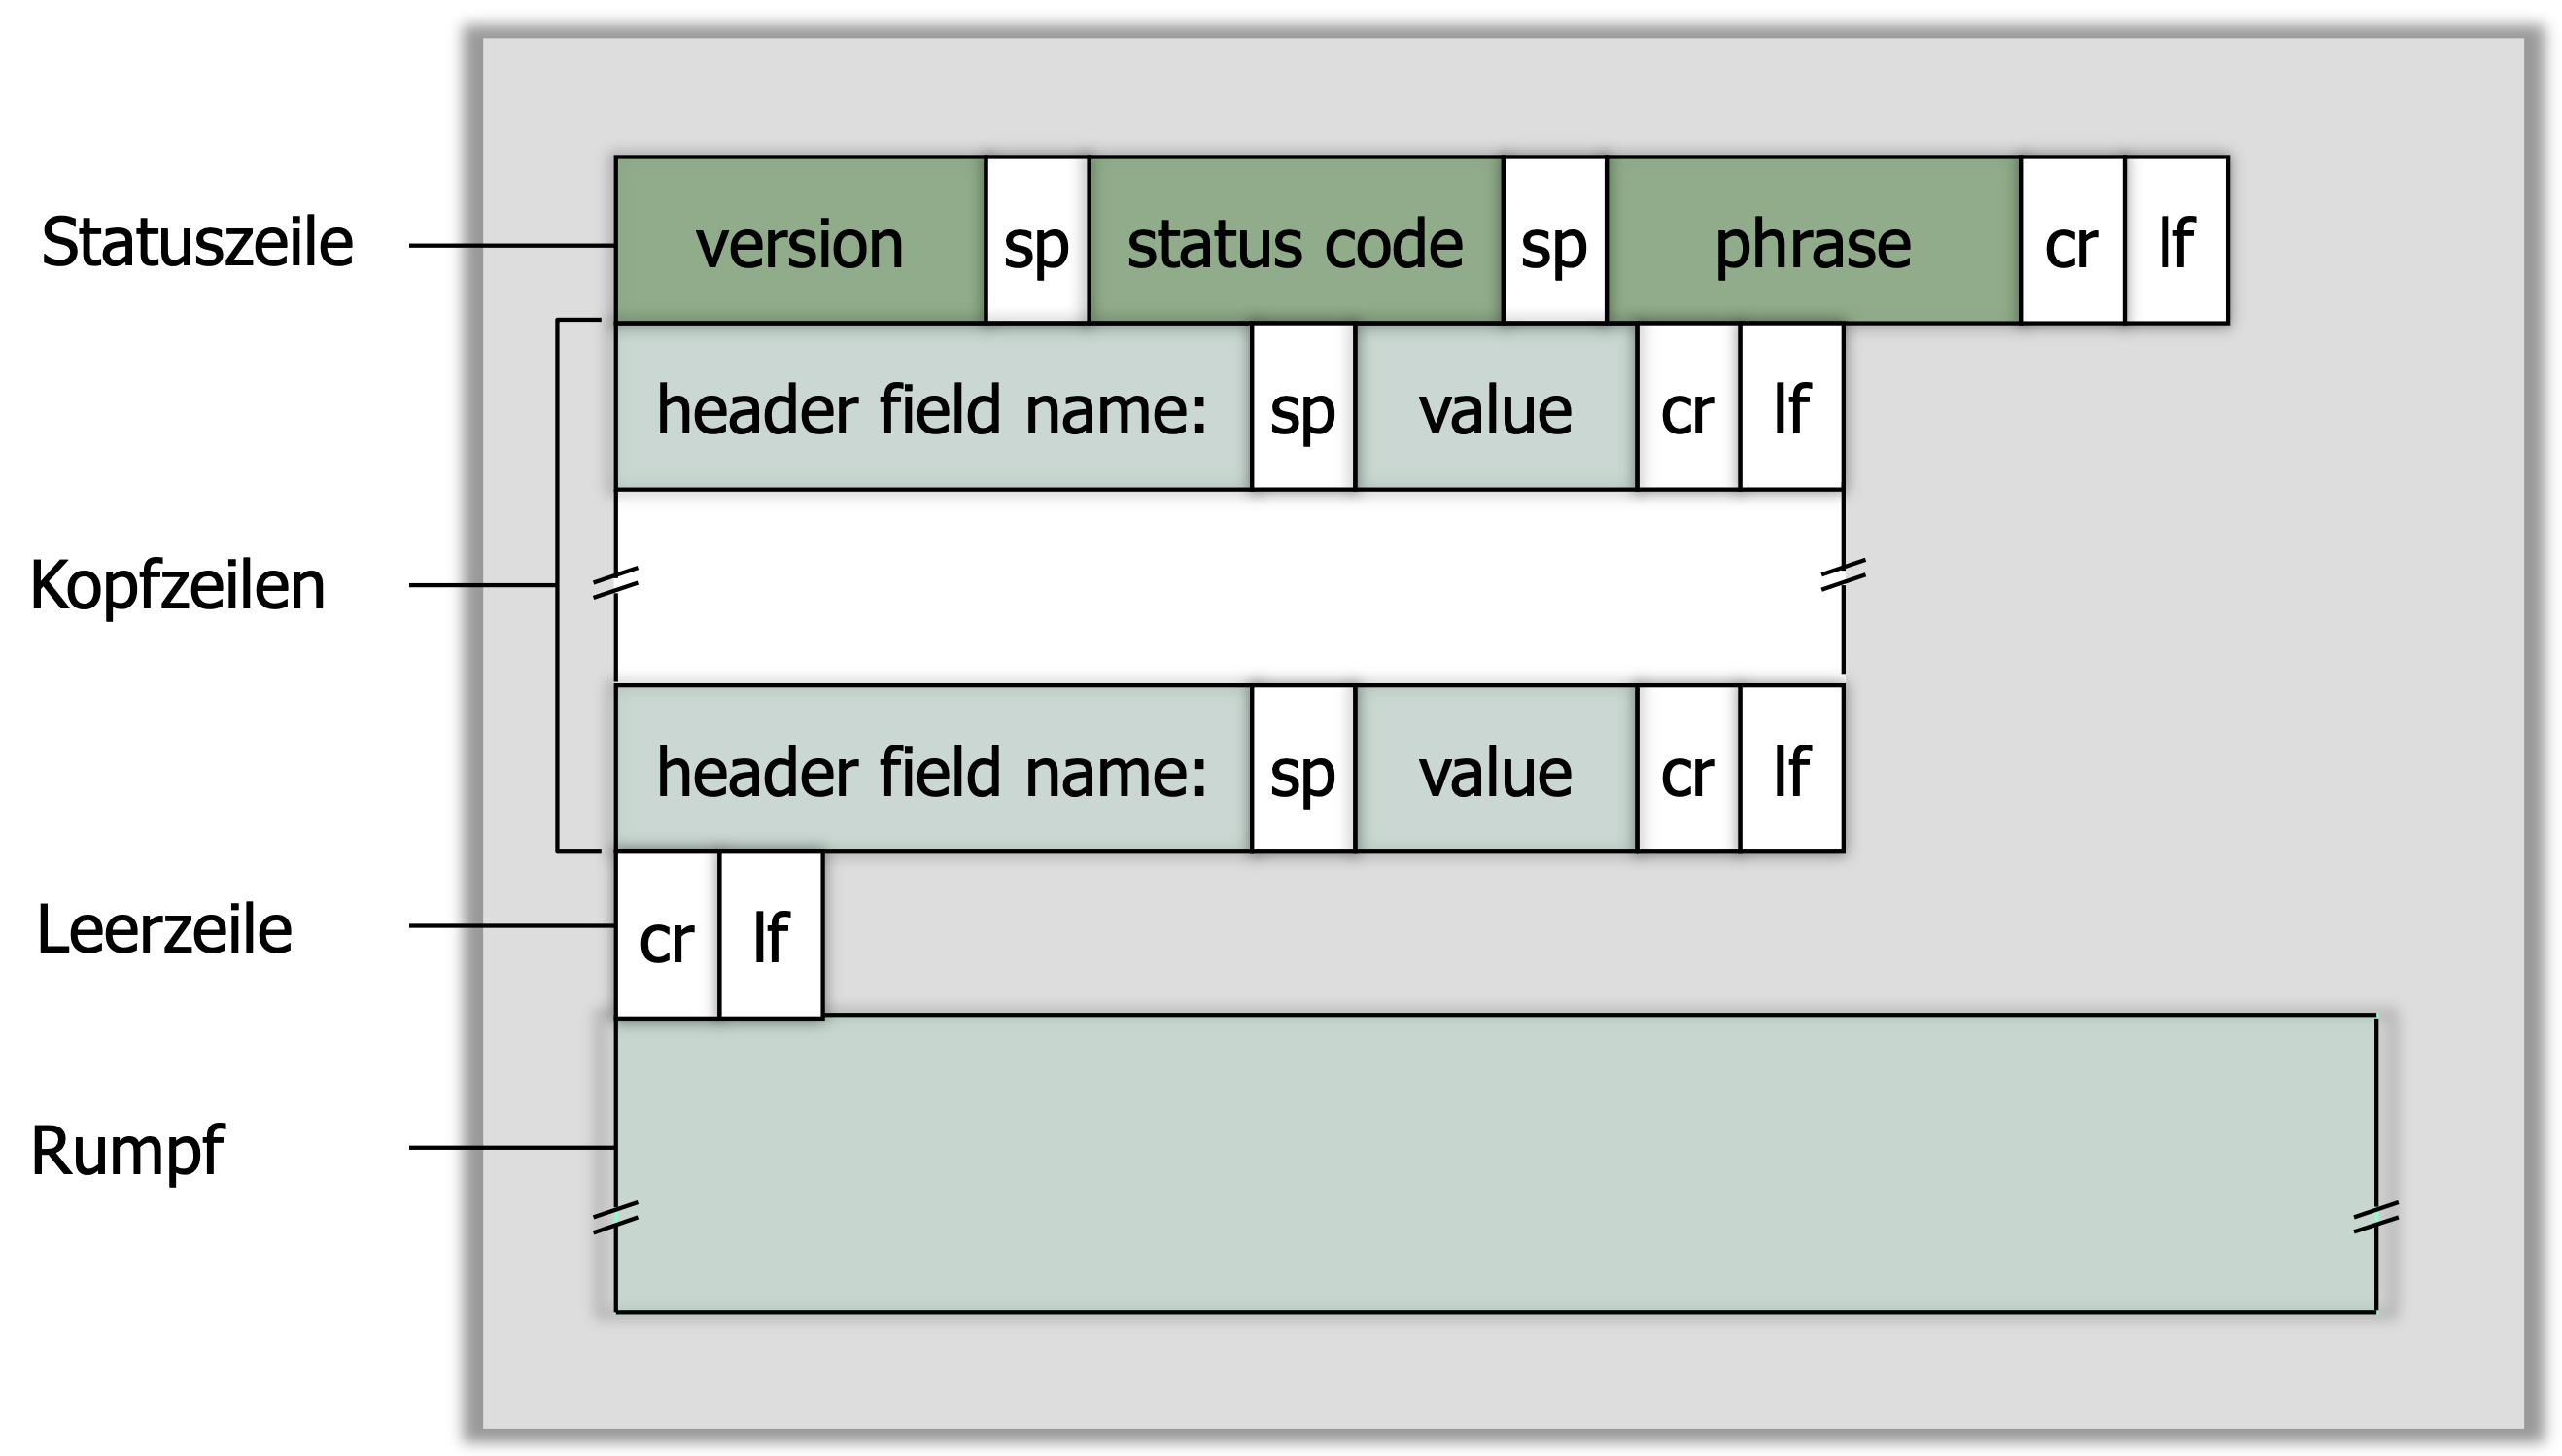
\includegraphics[scale=0.25]{Antwortnachricht_HTTP.png}
			\captionof{figure}{HTTP Antworten}
		\subsubsection{Antwortnachricht}
			\begin{center}
				\begin{tabular}{|cc|}
					\hline
					HTTP/1.1 & 200 OK \\
					Connection: & close \\
					Date: & Thu, 06 Aug 1998 12:00:15 GMT \\
					Server: & Apache/1.3.0 (Unix) \\
					Last-Modified: & Mon, 22 Jun 1998 ... \\
					Content-Length: & 6821 \\
					Content-Type: & text/html \\
					& \\
					data & data \\
					\hline
				\end{tabular}
				\captionof{figure}{Antwortnachricht}
			\end{center}
		\subsubsection{HTTP-Ablauf}
			\textbf{Nicht-persistentes HTTP}: \newline
				Für jedes Objekt wird eine einzelne TCP-Verbindung aufgebaut. Entweder Basisseite und eingebettete Objekte sequentiell oder parallele Verbindung für eingebettete Objekte
				\newline \newline
			\textbf{Persistentes HTTP}: \newline
				Server lässt Verbindung bestehen, alle Objekte werden über eine TCP Verbindung gesendet. Ohne Pipelining wird jedes Objekt einzeln Angefragt, mit alle auf einmal
			
		\subsubsection{Antwortzeit}
			Basisseite: Aufbau der TCP-Verbindung (1x RTT) + Anfrage hin und Antwort zurück (1x RTT) $\Rarr$ 2RTT + Zeit zum Senden + weitere Wartezeiten durch TCP \newline
			\begin{center}
				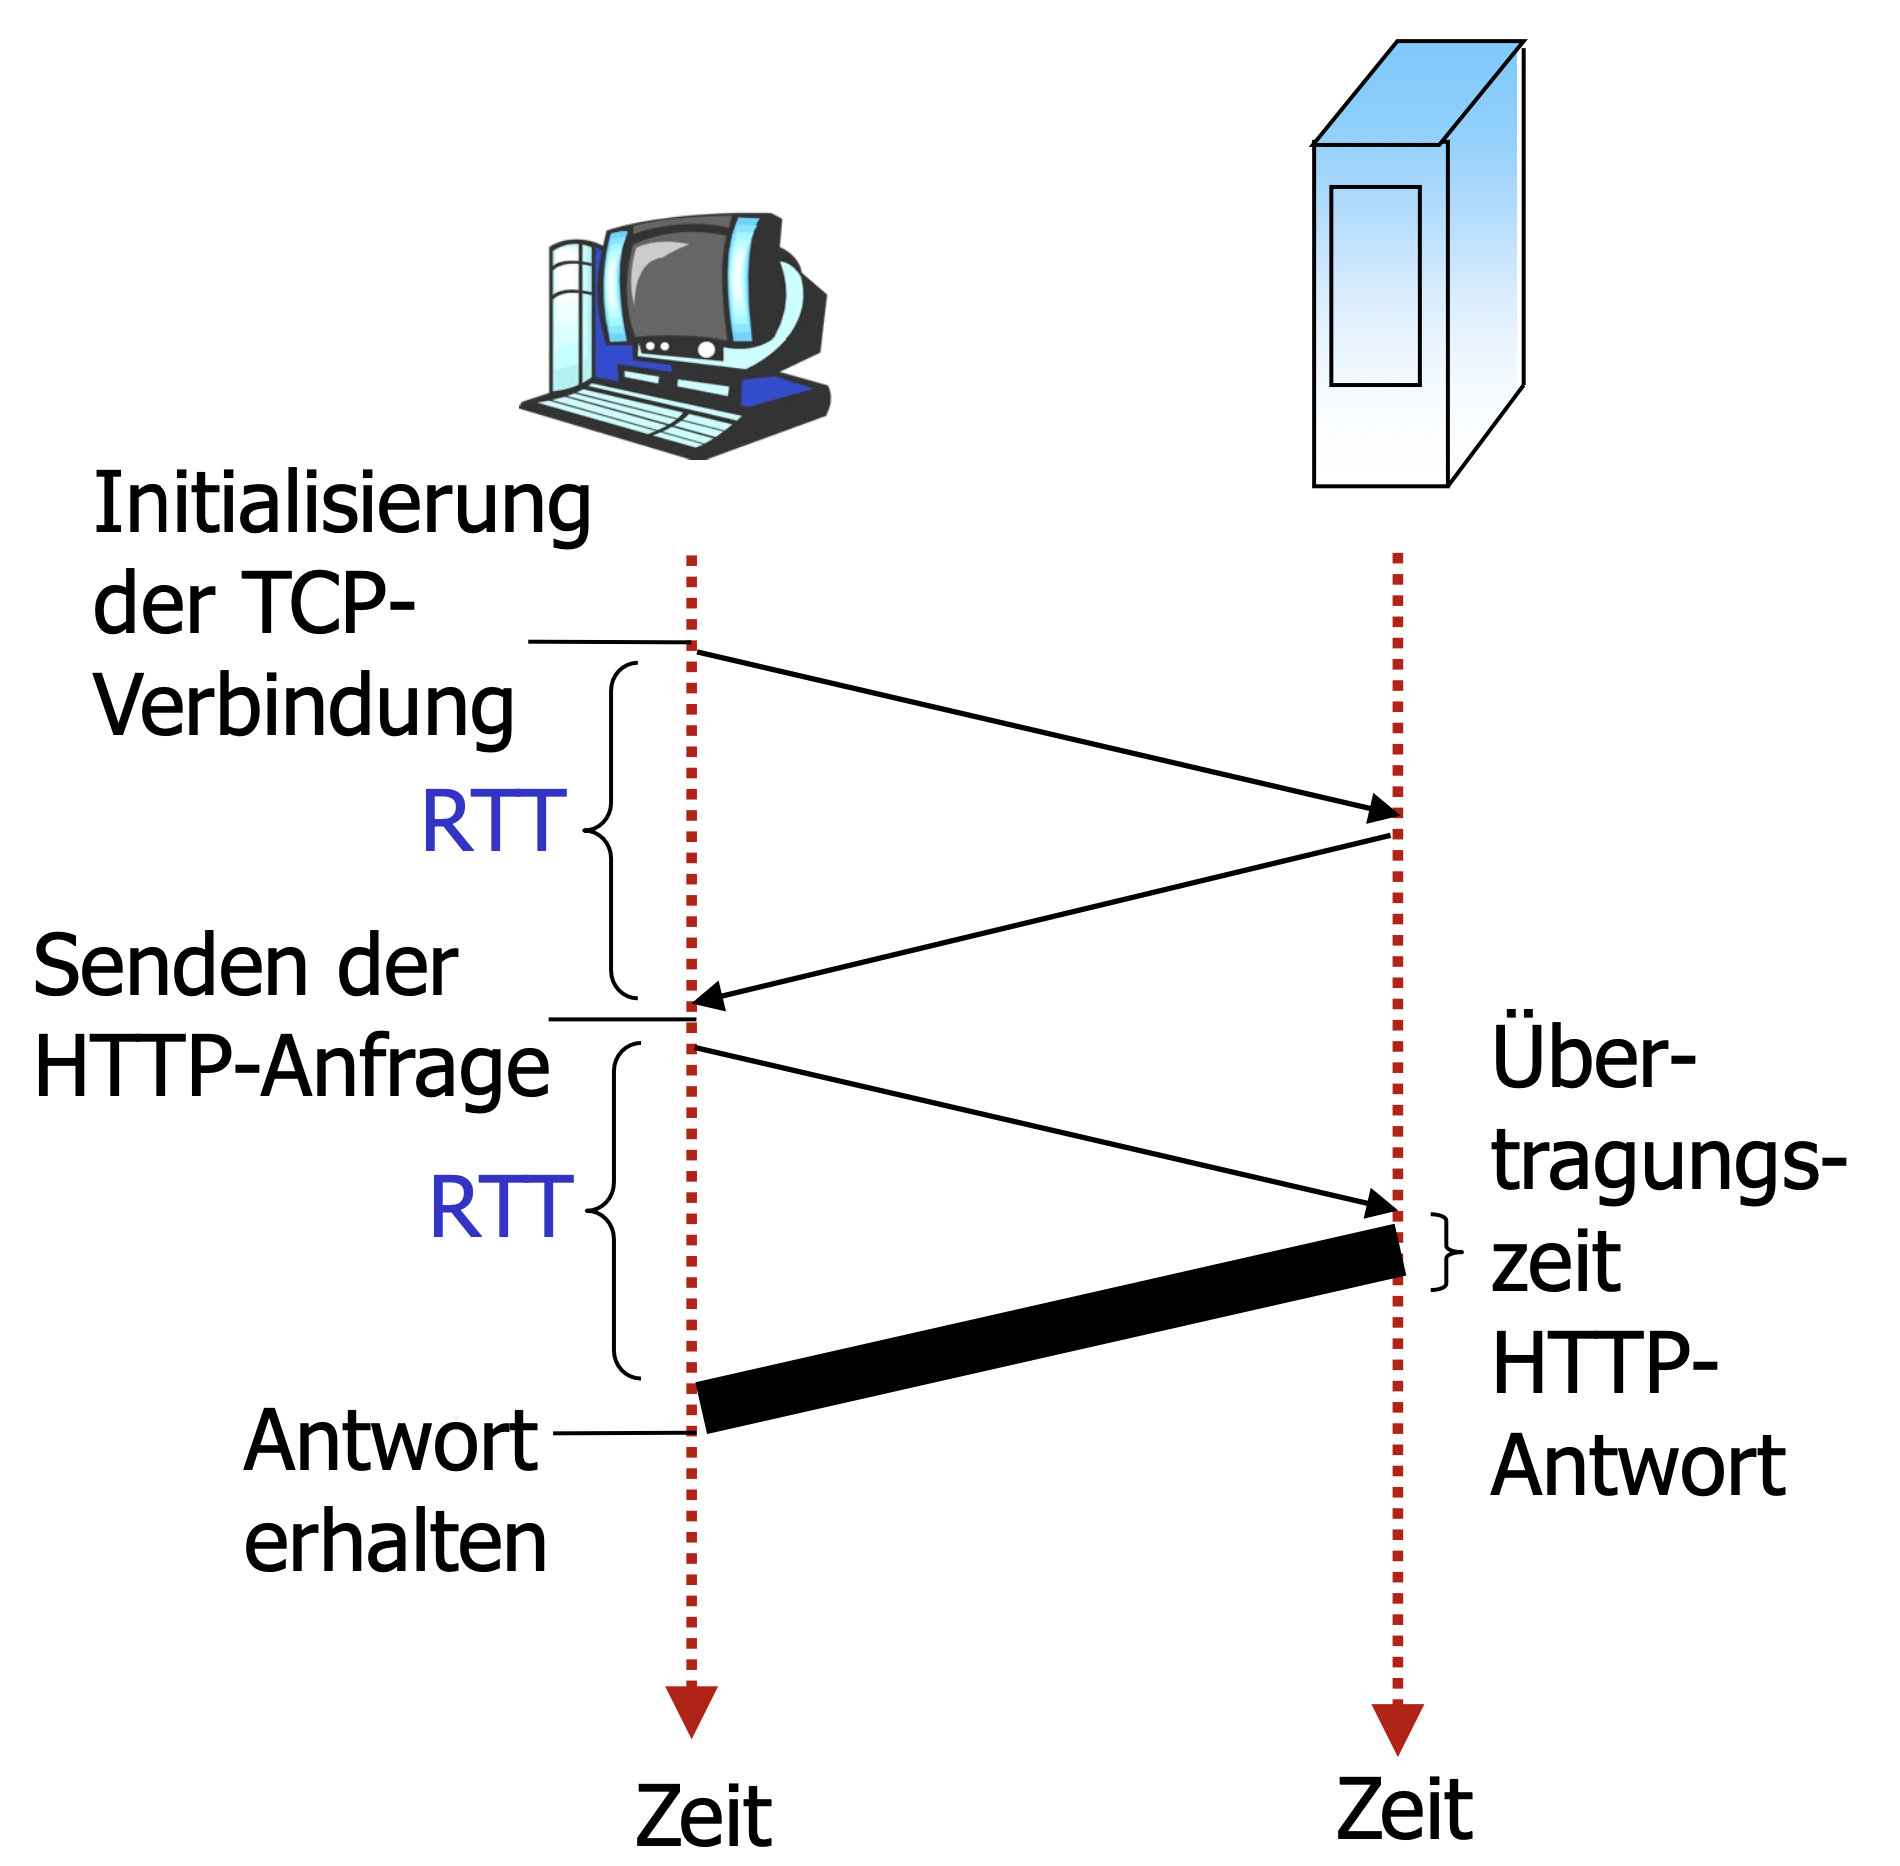
\includegraphics[scale=0.25]{Antwortzeit_HTTP_Basis.png}	
				\captionof{figure}{Antwortzeit}
			\end{center}
		\subsubsection{Dynamische Inhalte}
			\textbf{Common Gate Interface (CGI)} verarbeitet als externer Prozess die Information und liefert neue HTML-Seite an Server \newline \newline
			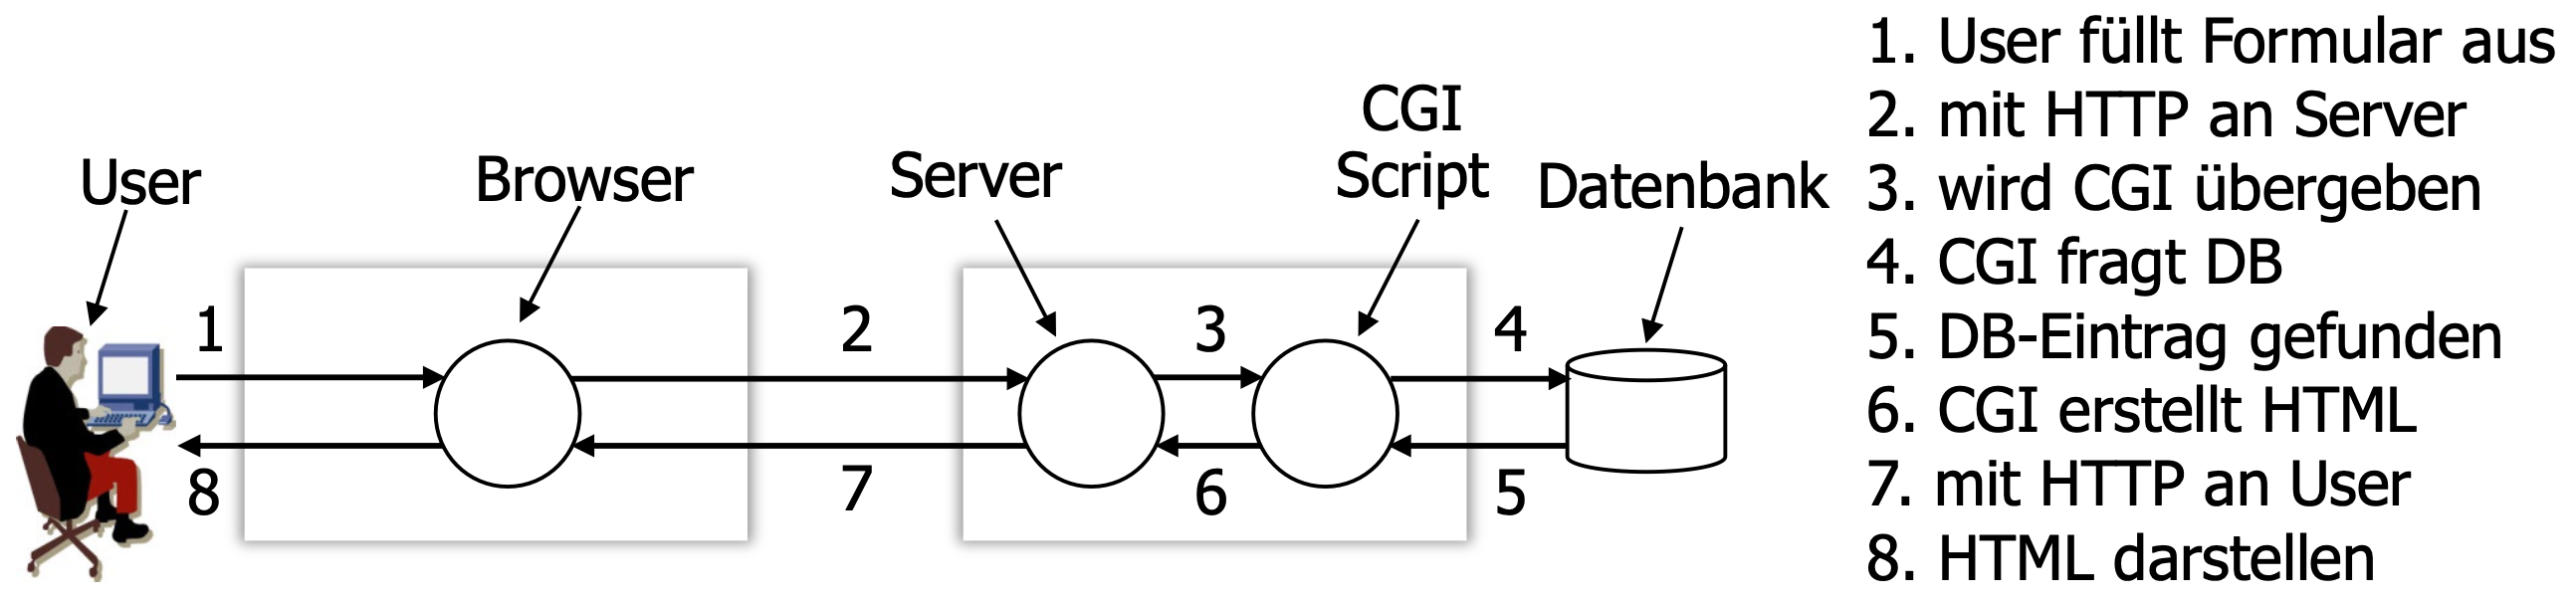
\includegraphics[scale=0.25]{CGI_HTML.png}
			\captionof{figure}{CGI}
			\textbf{Scripting:} Durch Interpretation von eingebetteten Skripten können dynamische Inhalte erzeugt werden.\newline \newline
			Serverseitig: im HTML ist Code eingebettet, der vom Server interpretiert wird und dabei HTML erzeugt, z.B. PHP \newline \newline
			Clientseitig: im HTML ist Code eingebettet, der vom Client interpretiert wird, z.B. JavaScript
		\subsubsection{Caching}
			Cache (Proxy Server) ist Server für Web-Browser und Client für Web-Server, der als Zwischenspeicher zur Verringerung der Wartezeit des Nutzers und des Netzverkehrs dient
			\begin{center}
				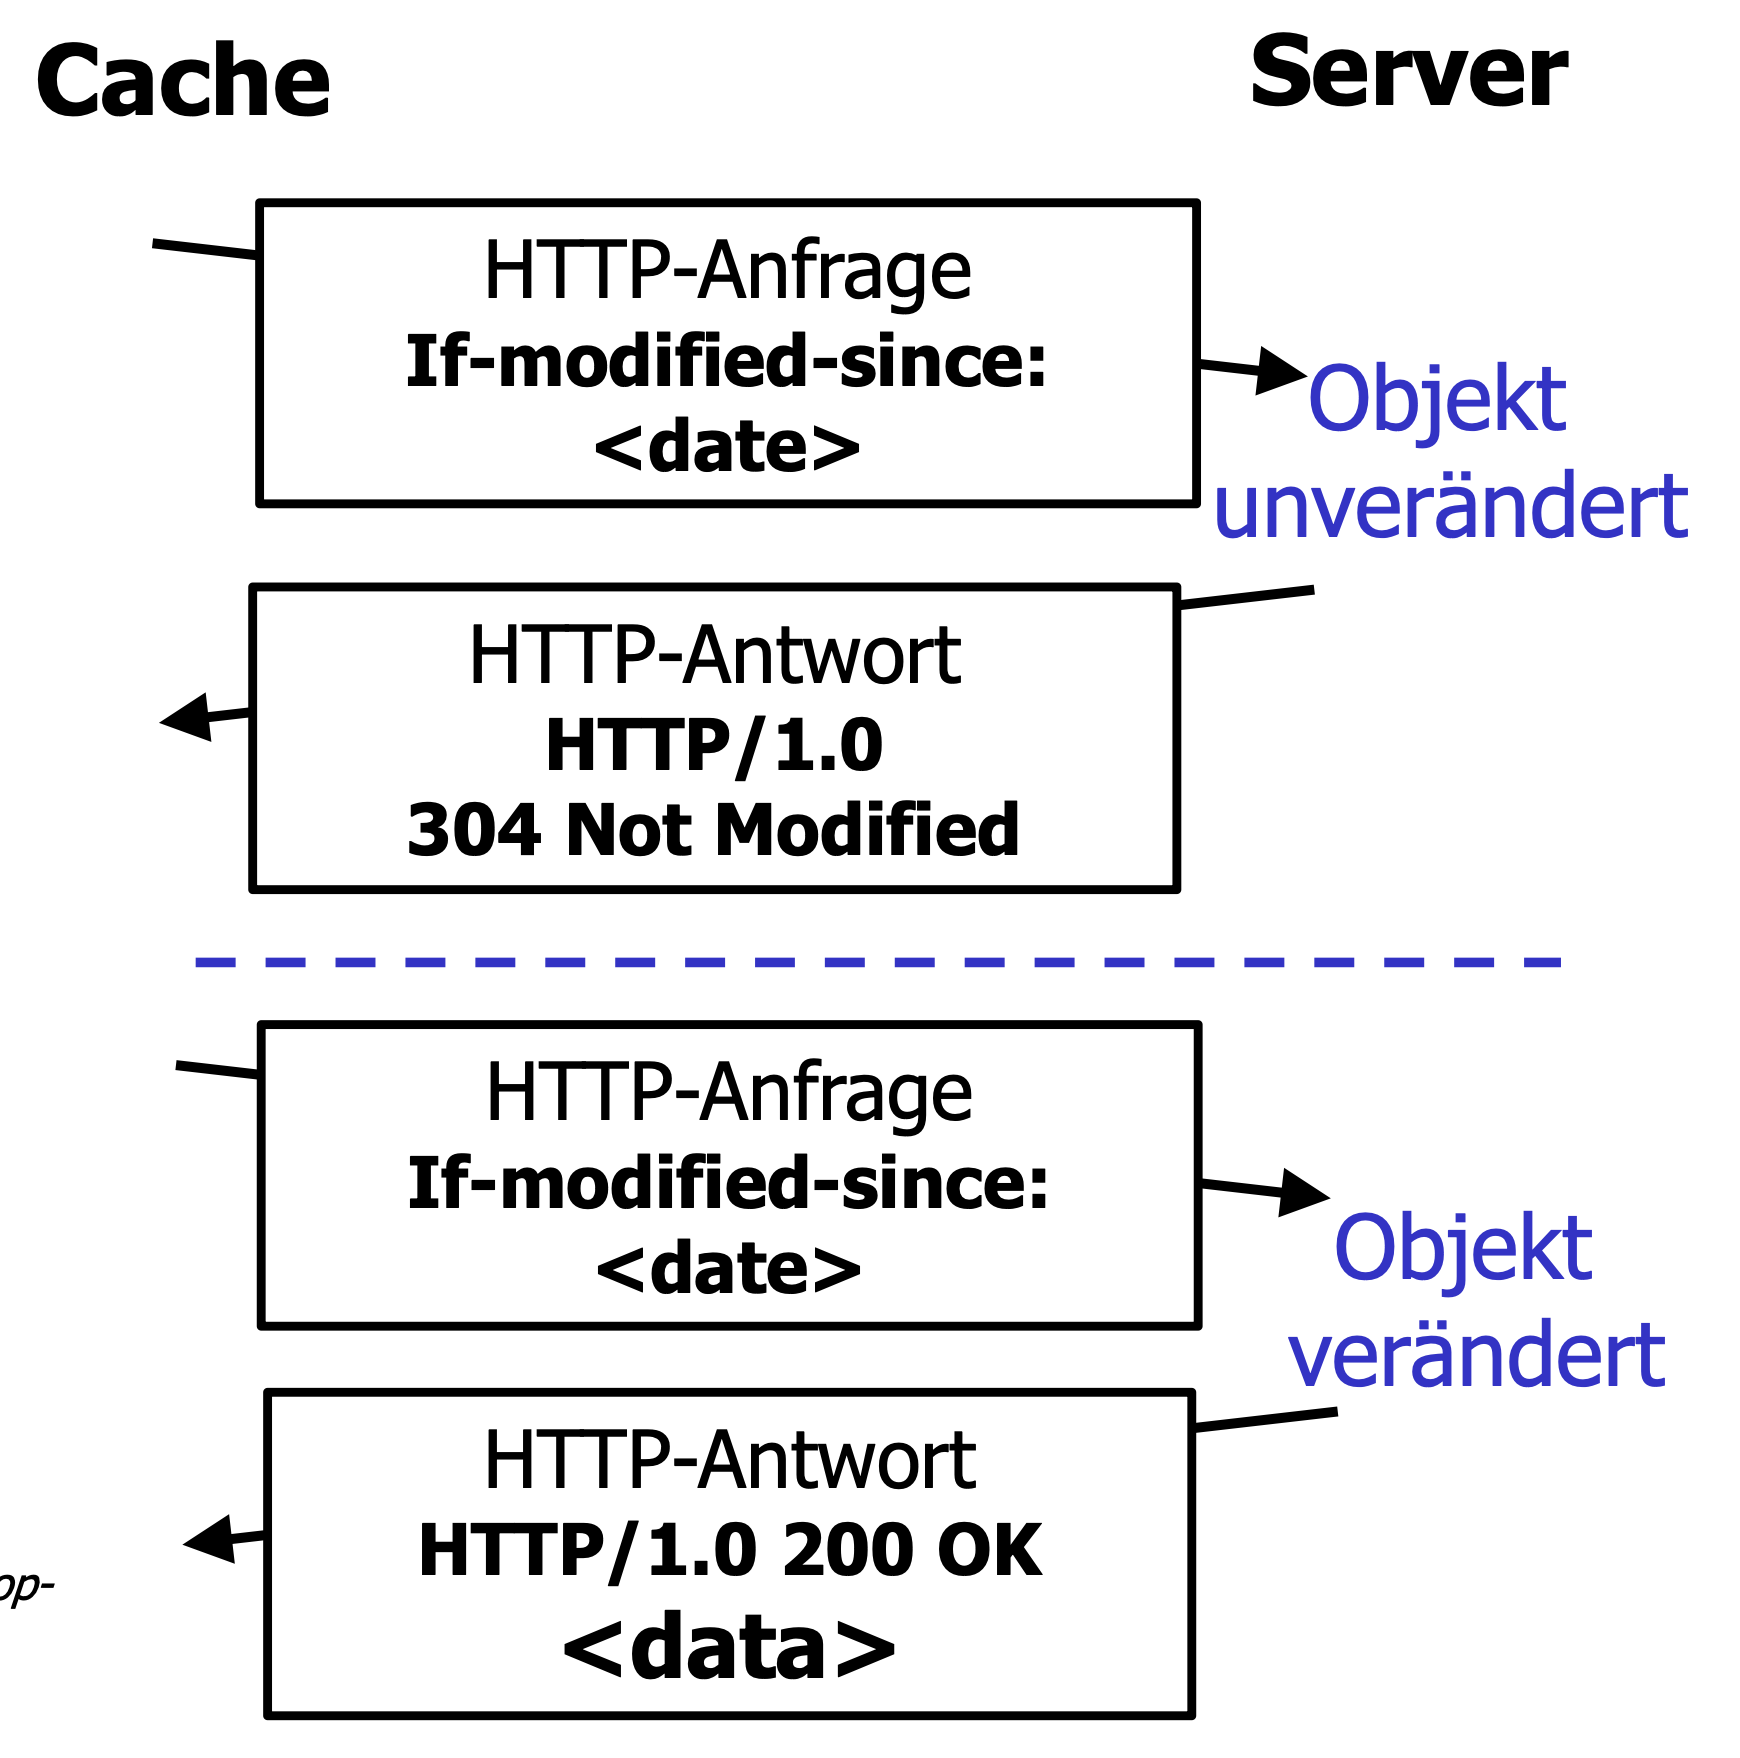
\includegraphics[scale=0.25]{Cache_Server_HTML.png}
				\captionof{figure}{Cache Server}
			\end{center}
		\subsubsection{HTTP/2}
			Wesentliche Elemente: 
			\begin{itemize}
				\item gleiche Methoden
				\item binäres statt textbasiertes Format
				\item Multiplexing verschiedener Ströme über eine TCP-Verbindung, Vermeidung von Head-of-Line (HOL) Blockierung durch große Objekte durch Aufteilung in kleinere Frames und Interleaving
				\item Header-Kompression
				\item Server-Push
			\end{itemize}
	\subsection{File Transfere Protocol (FTP)}
		\begin{itemize}
			\item Übertragung zwischen zwei Hosts
			\item eine TCP-Verbindung (Port 21) zur Steuerung
			\item lesbare Kommandos: USER username, PASS password, LIST, PETR filename, STOR filename, ...
			\item jeweils eine TCP-Verbindung (Port 20) zur  Übertragung einer Datei
			\item 'out-of-band-controll'
		\end{itemize}
		\begin{center}
			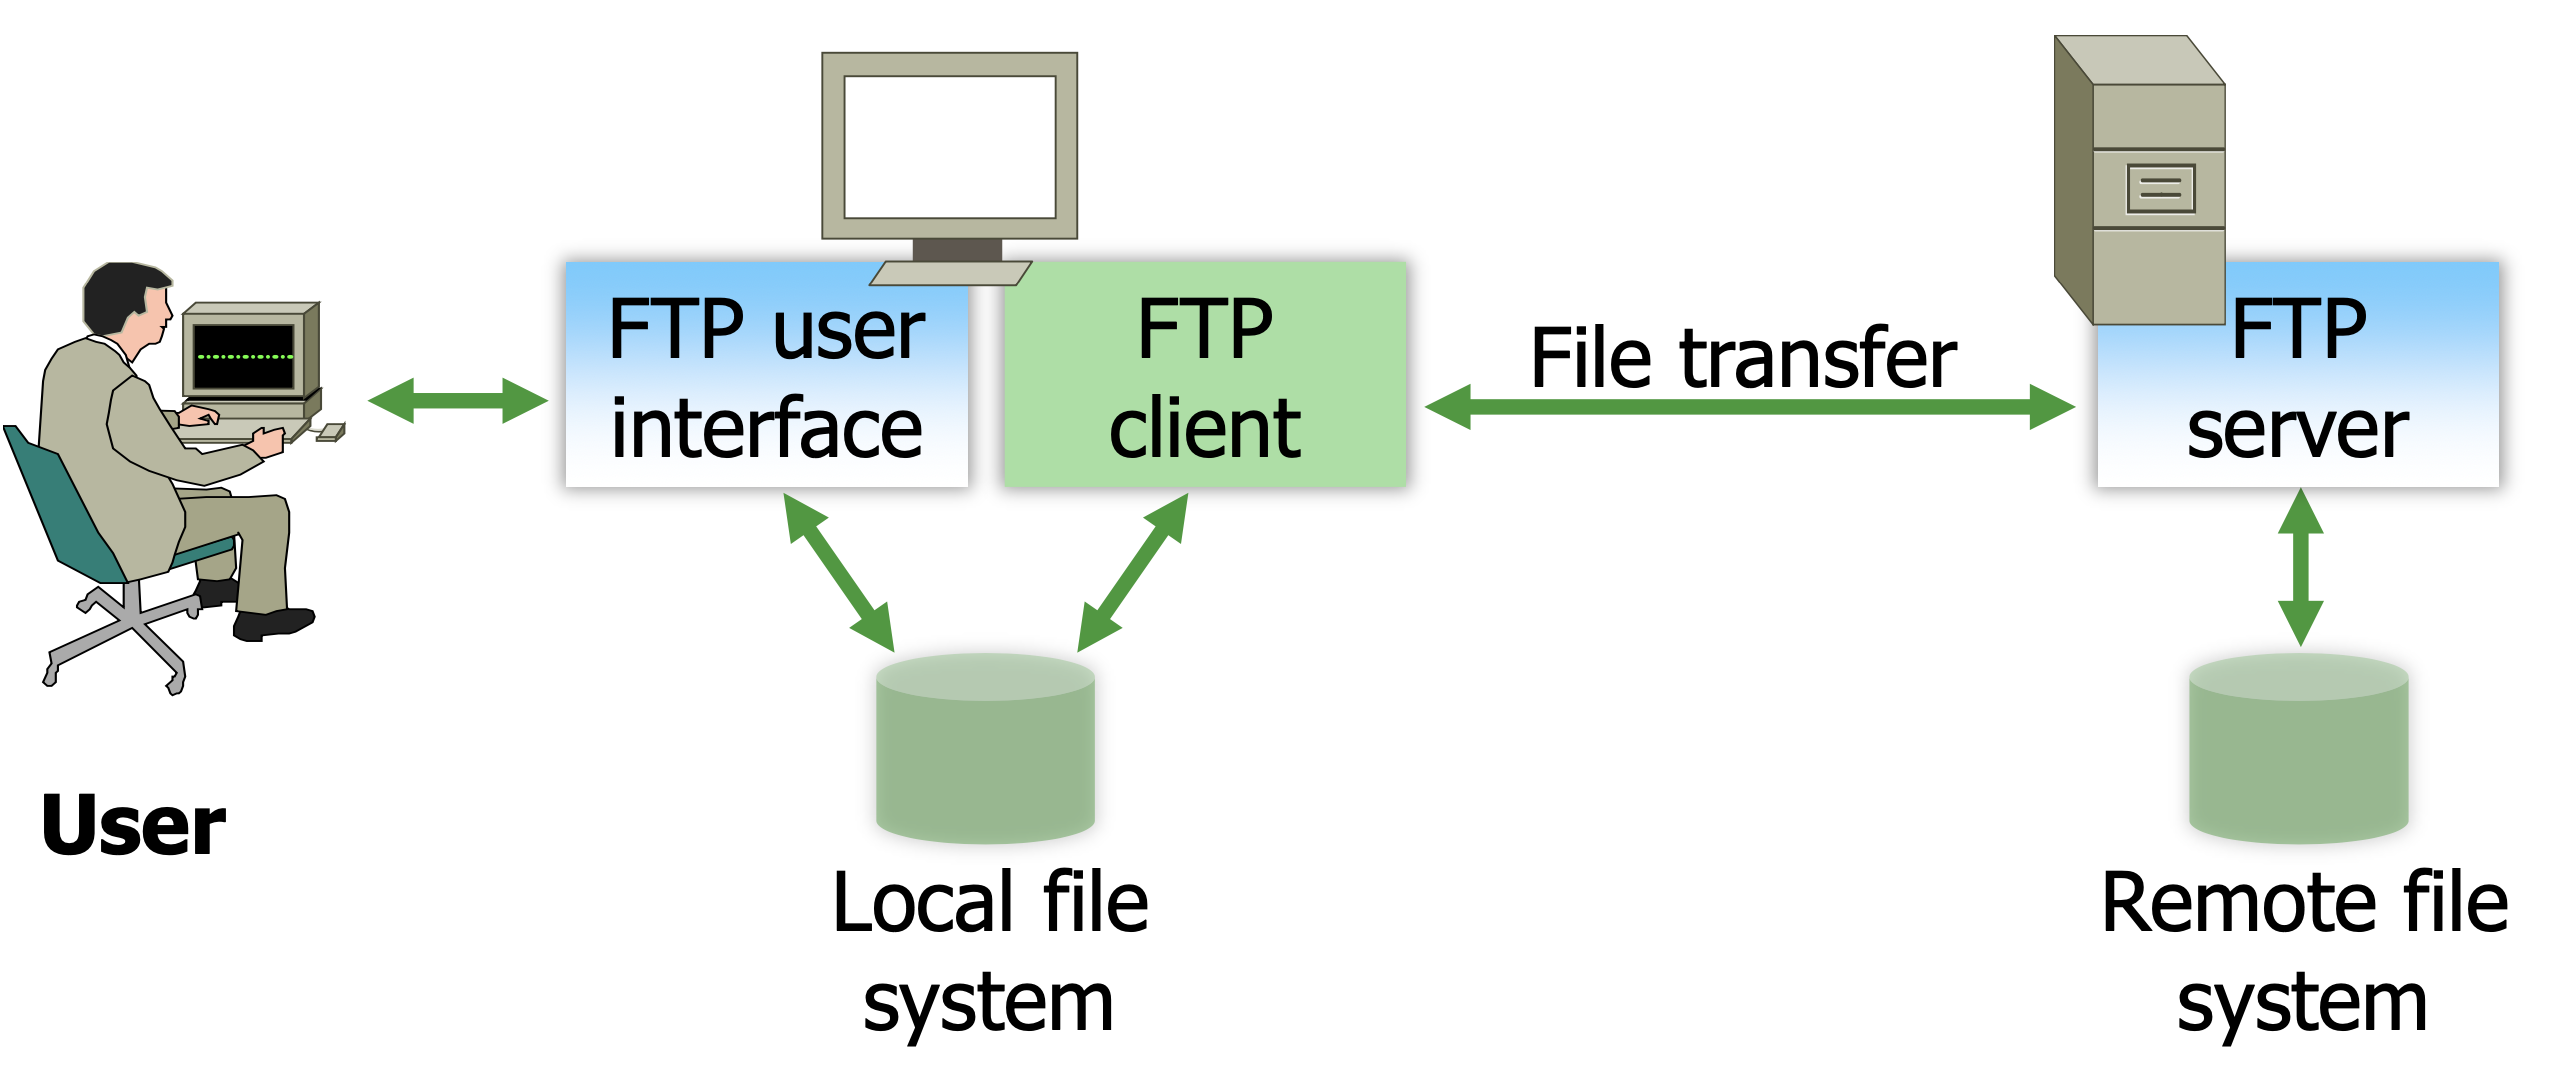
\includegraphics[scale=0.25]{FTP.png}
			\captionof{figure}{FTP}
		\end{center}
	\subsection{Simple Mail Transfer Protocol (SMTP)}
		\begin{itemize}
			\item Nachrichten im ASCII-Format, Kopf, Rumpf
			\item andere Daten werden in ASCII umgewandelt angehängt
			\item Versenden mit SMPT über TCP (lesbar)
			\item Abholen mit POP3, IMAP, HTTP (lesbar)
		\end{itemize}
		\begin{center}
			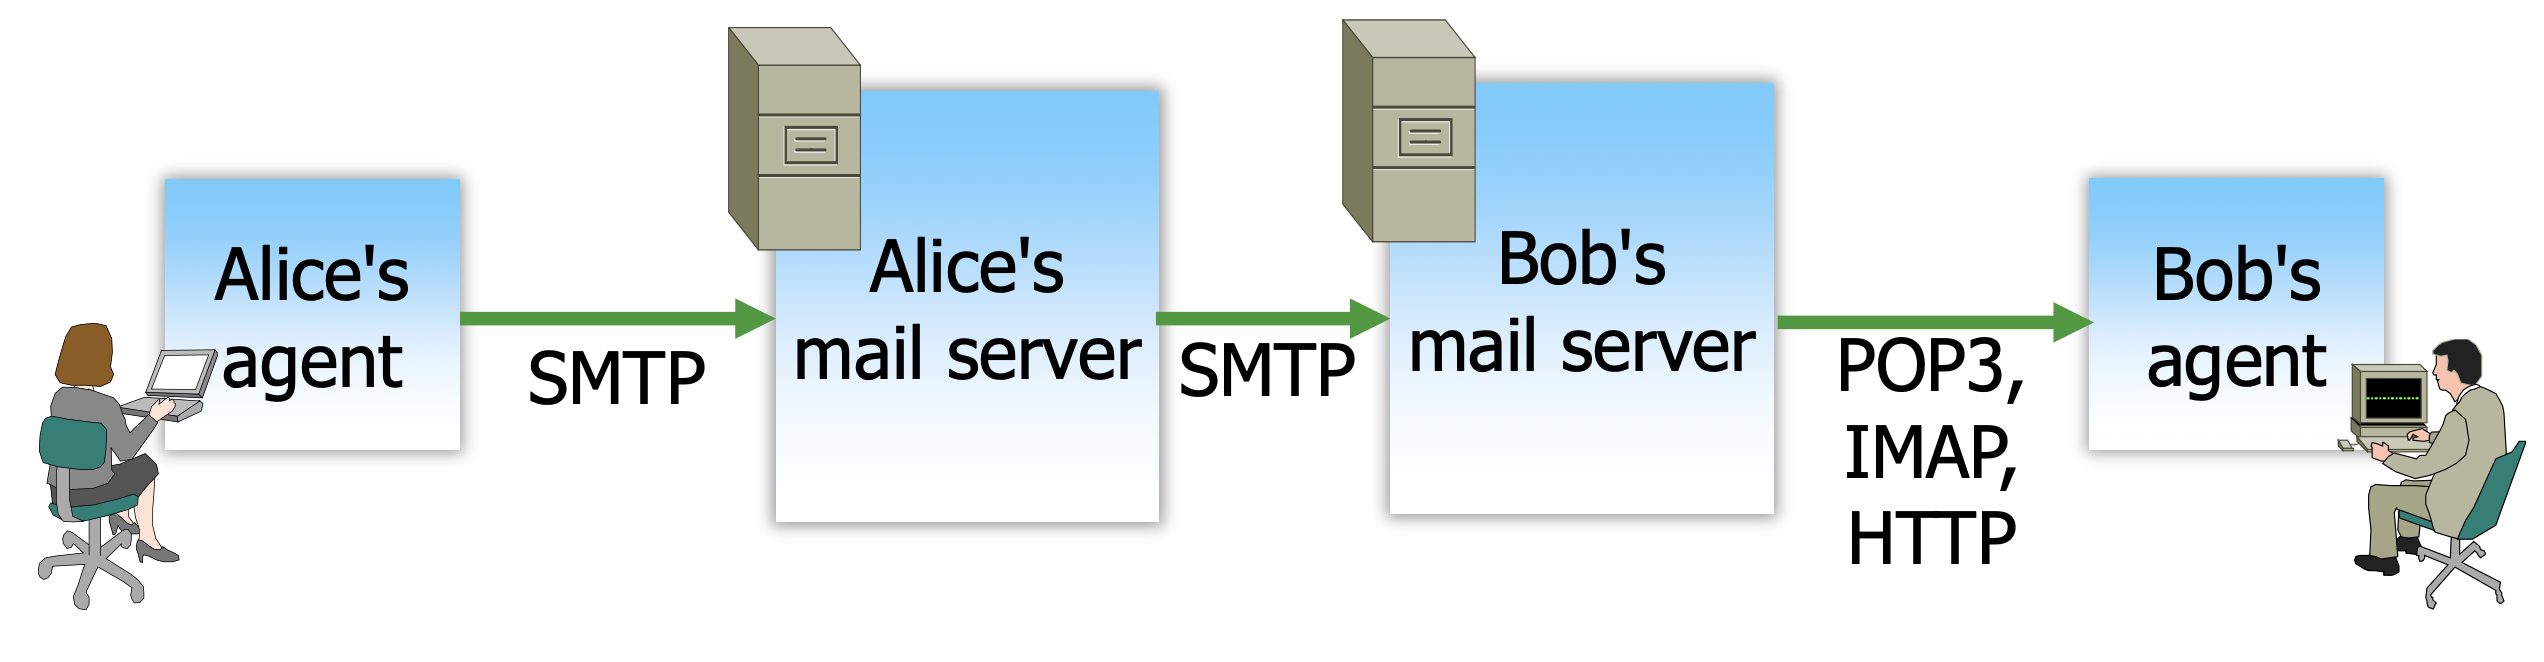
\includegraphics[scale=0.25]{SMTP.png}
			\captionof{figure}{SMTP}
		\end{center}
		\begin{itemize}
			\item nutzt TCP (Port 25)
			\item direkte Übertragung: vom Sendenden zu empfangendem Server
			\item drei Phasen der Übertragung:
				\begin{itemize}
					\item Handshake
					\item Nachrichtenübertragung
					\item Abschlussphase
				\end{itemize}
			\item Interaktion mittels Befehlen und Antworten
				\begin{itemize}
					\item Befehle: ASCII-text
					\item Antworten: Statuscode und Text
				\end{itemize}
			\item Nachrichten müssen 7-bit ASCII-text sein
		\end{itemize}
		\subsubsection{Vertraulichkeit und Datenintegrität}
			\begin{enumerate}
				\item Erzeugung eines Hashwerts der E-Mail
				\item Signierung mit privatem Schlüssel $K_A^-$ von Alice
				\item Verschlüsselung der Mail und der Signatur mit $K_S$
				\item Asymmetrische Verschlüsselung von $K_S$ mit dem öffentlichen Schlüssel $K_B^+$ von Bob
			\end{enumerate}
			\begin{center}
				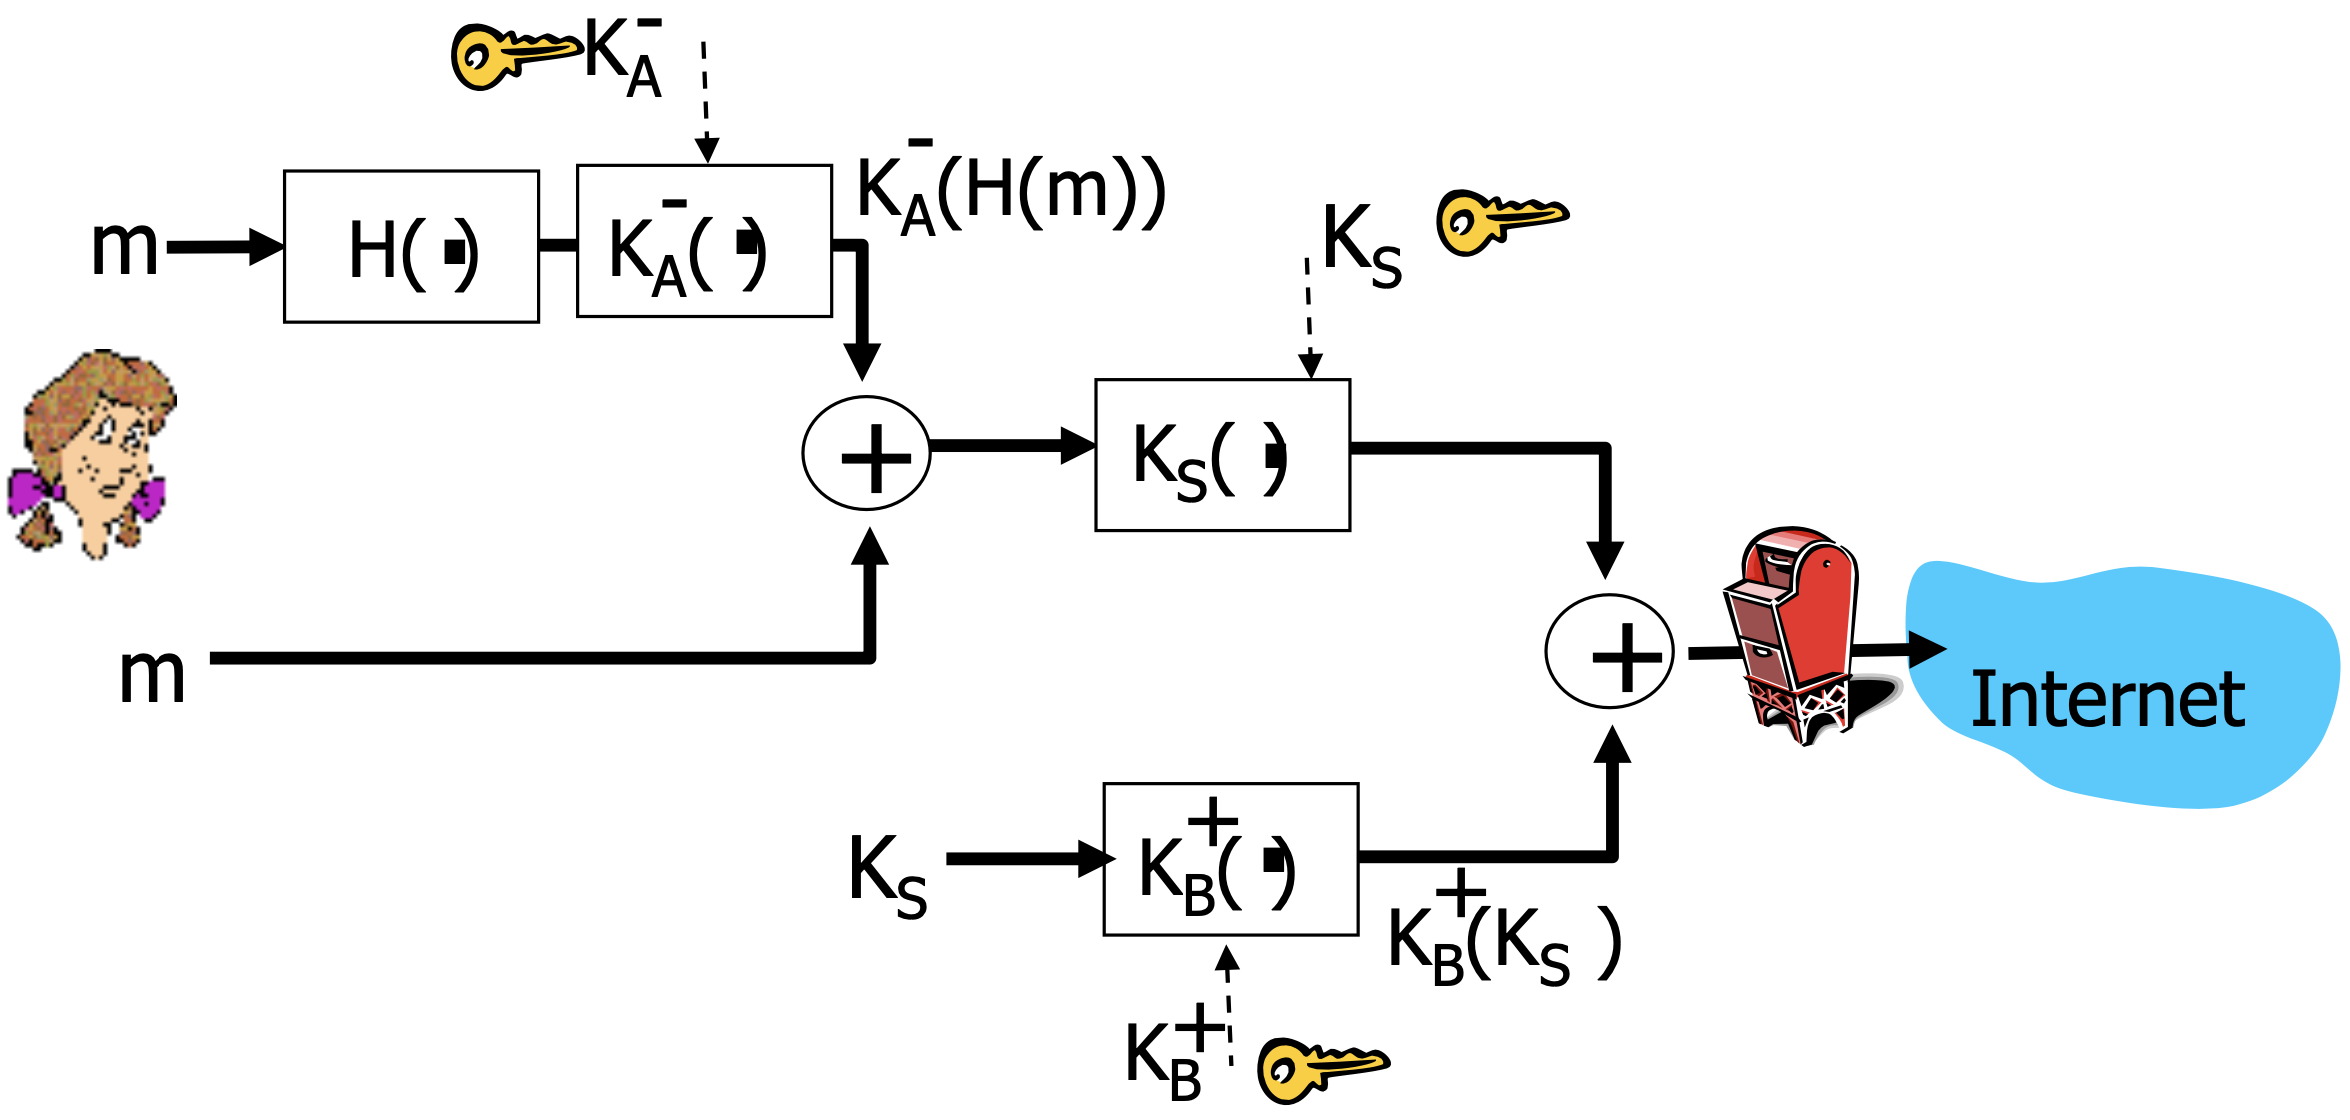
\includegraphics[scale=0.25]{Sicherheit_SMPT.png}
				\captionof{figure}{Vertraulichkeit und Datenintegrität}
			\end{center}

	
	\subsection{Netzwerkmanagement}
		Überwachung und Verwaltung eines Netzes = komplexes HW/SW Gebilde \newline
		FCAPS-Modell nach ISO:
		\begin{itemize}
			\item Fault Management: Monitoring, Dokumentation, Reaktionsmaßnahmen
			\item Configuration Management: Übersicht über Geräte und deren HW/SW-Konfigurationen 
			\item Accounting Management: Verwendung von Netzwerkressourcen, Festlegung, Kontrolle, Dokumentation des Zugangs von Benutzern und Geräten
			\item Performance Management: Monitoring von Auslastung, Durchsatz, Antwortzeiten, Dokumentation, Reaktionsmaßnahmen
			\item Security Management: Monitoring und Kontrolle des Zugangs, Schlüsselverwaltung, Firewalls, Intrusion Detection
		\end{itemize}
		\subsubsection{Simple Network Management Protocol (SNMP)}
			Organisationsmodell: 
			\begin{itemize}
				\item Managing Entity: Prozess auf zentraler Management Station, Client
				\item Managed Device
				\item Managed Object: HW oder SW im Managed Device
				\item Managed Agent: Prozess auf Managed Device, kann lokal ausgeführt werden
				\item Anfrage/Antwort-Protokoll zwischen Manager und Agent über UDP
				\item Manager basierend auf Regeln, was zu tun ist
			\end{itemize}
			\begin{center}
				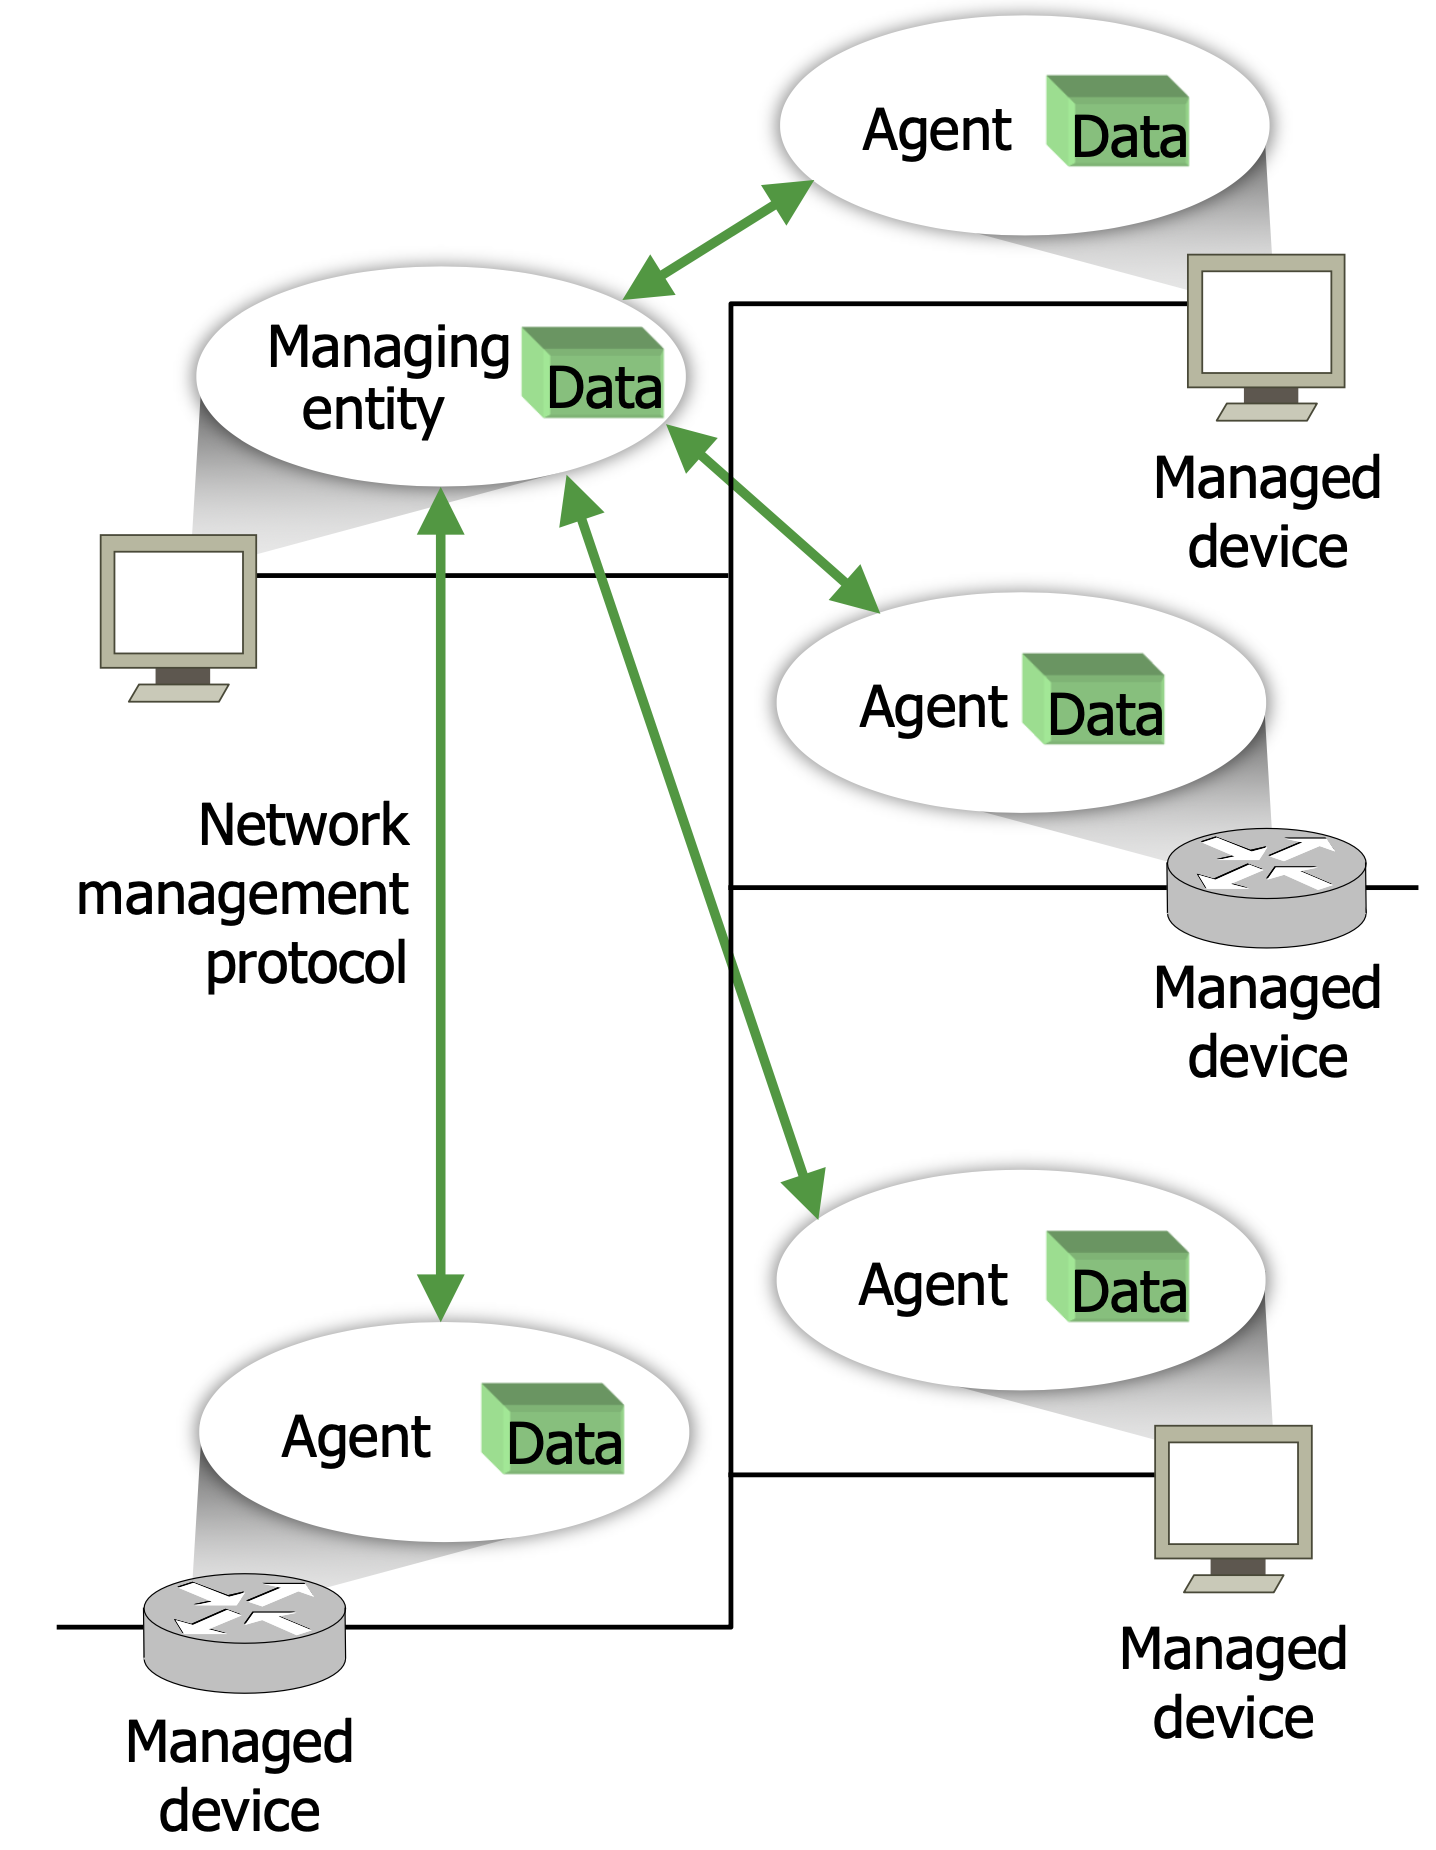
\includegraphics[scale=0.25]{SNMP.png}
				\captionof{figure}{SNMP}
			\end{center}
			SNMP Messages:
			\begin{itemize}
				\item \textbf{Get}: Manager an Agent, um Daten von Agent zu erhalten
				\item \textbf{Get-Next}: Manager an Agent, für nächsten Datensatz, Zugriff auf sequentielle Datensätze
				\item \textbf{Get-Bulck}: Manager an Agent, für mehrere Datensätze auf einmal
				\item \textbf{Set}: Manager an Agent, initialisiert oder ändert den Wert eines Datensatzes 
				\item \textbf{Response}: Agent an Manager, Antwort auf Get- und Set-Nachrichten
				\item \textbf{Trap}: Agent an Manager, unaufgeforderte Nachricht über Fehlersituation
			\end{itemize}
			\begin{center}
				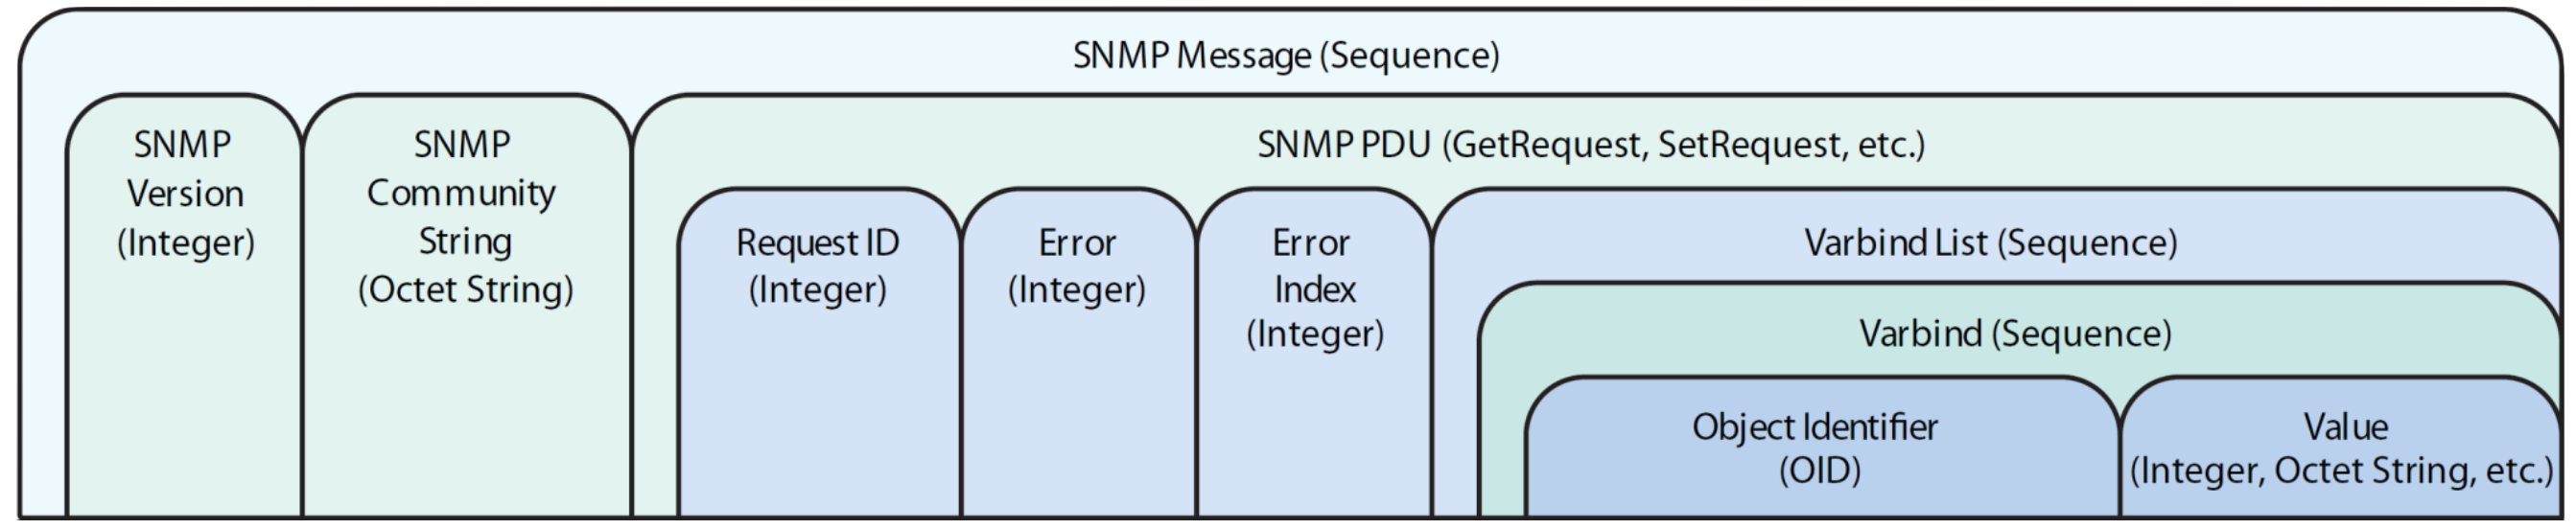
\includegraphics[scale=0.25]{SNMP_Nachrichten.png}
				\captionof{figure}{Format von SNMP Nachrichten}
			\end{center}
		\subsubsection{Management Information Base (MIB)}
			MIB-Module enthalten Datenstrukturen für die Managed Devices. Das genaue binäre Format der Übertragung wird mit Basic Encoding Rules (BER) festgestellt. Jedes MIB-Modul wird eindeutig durch die Objekt-Identifizierung (OID) der ASN.1 bezeichnet.
			\begin{center}
				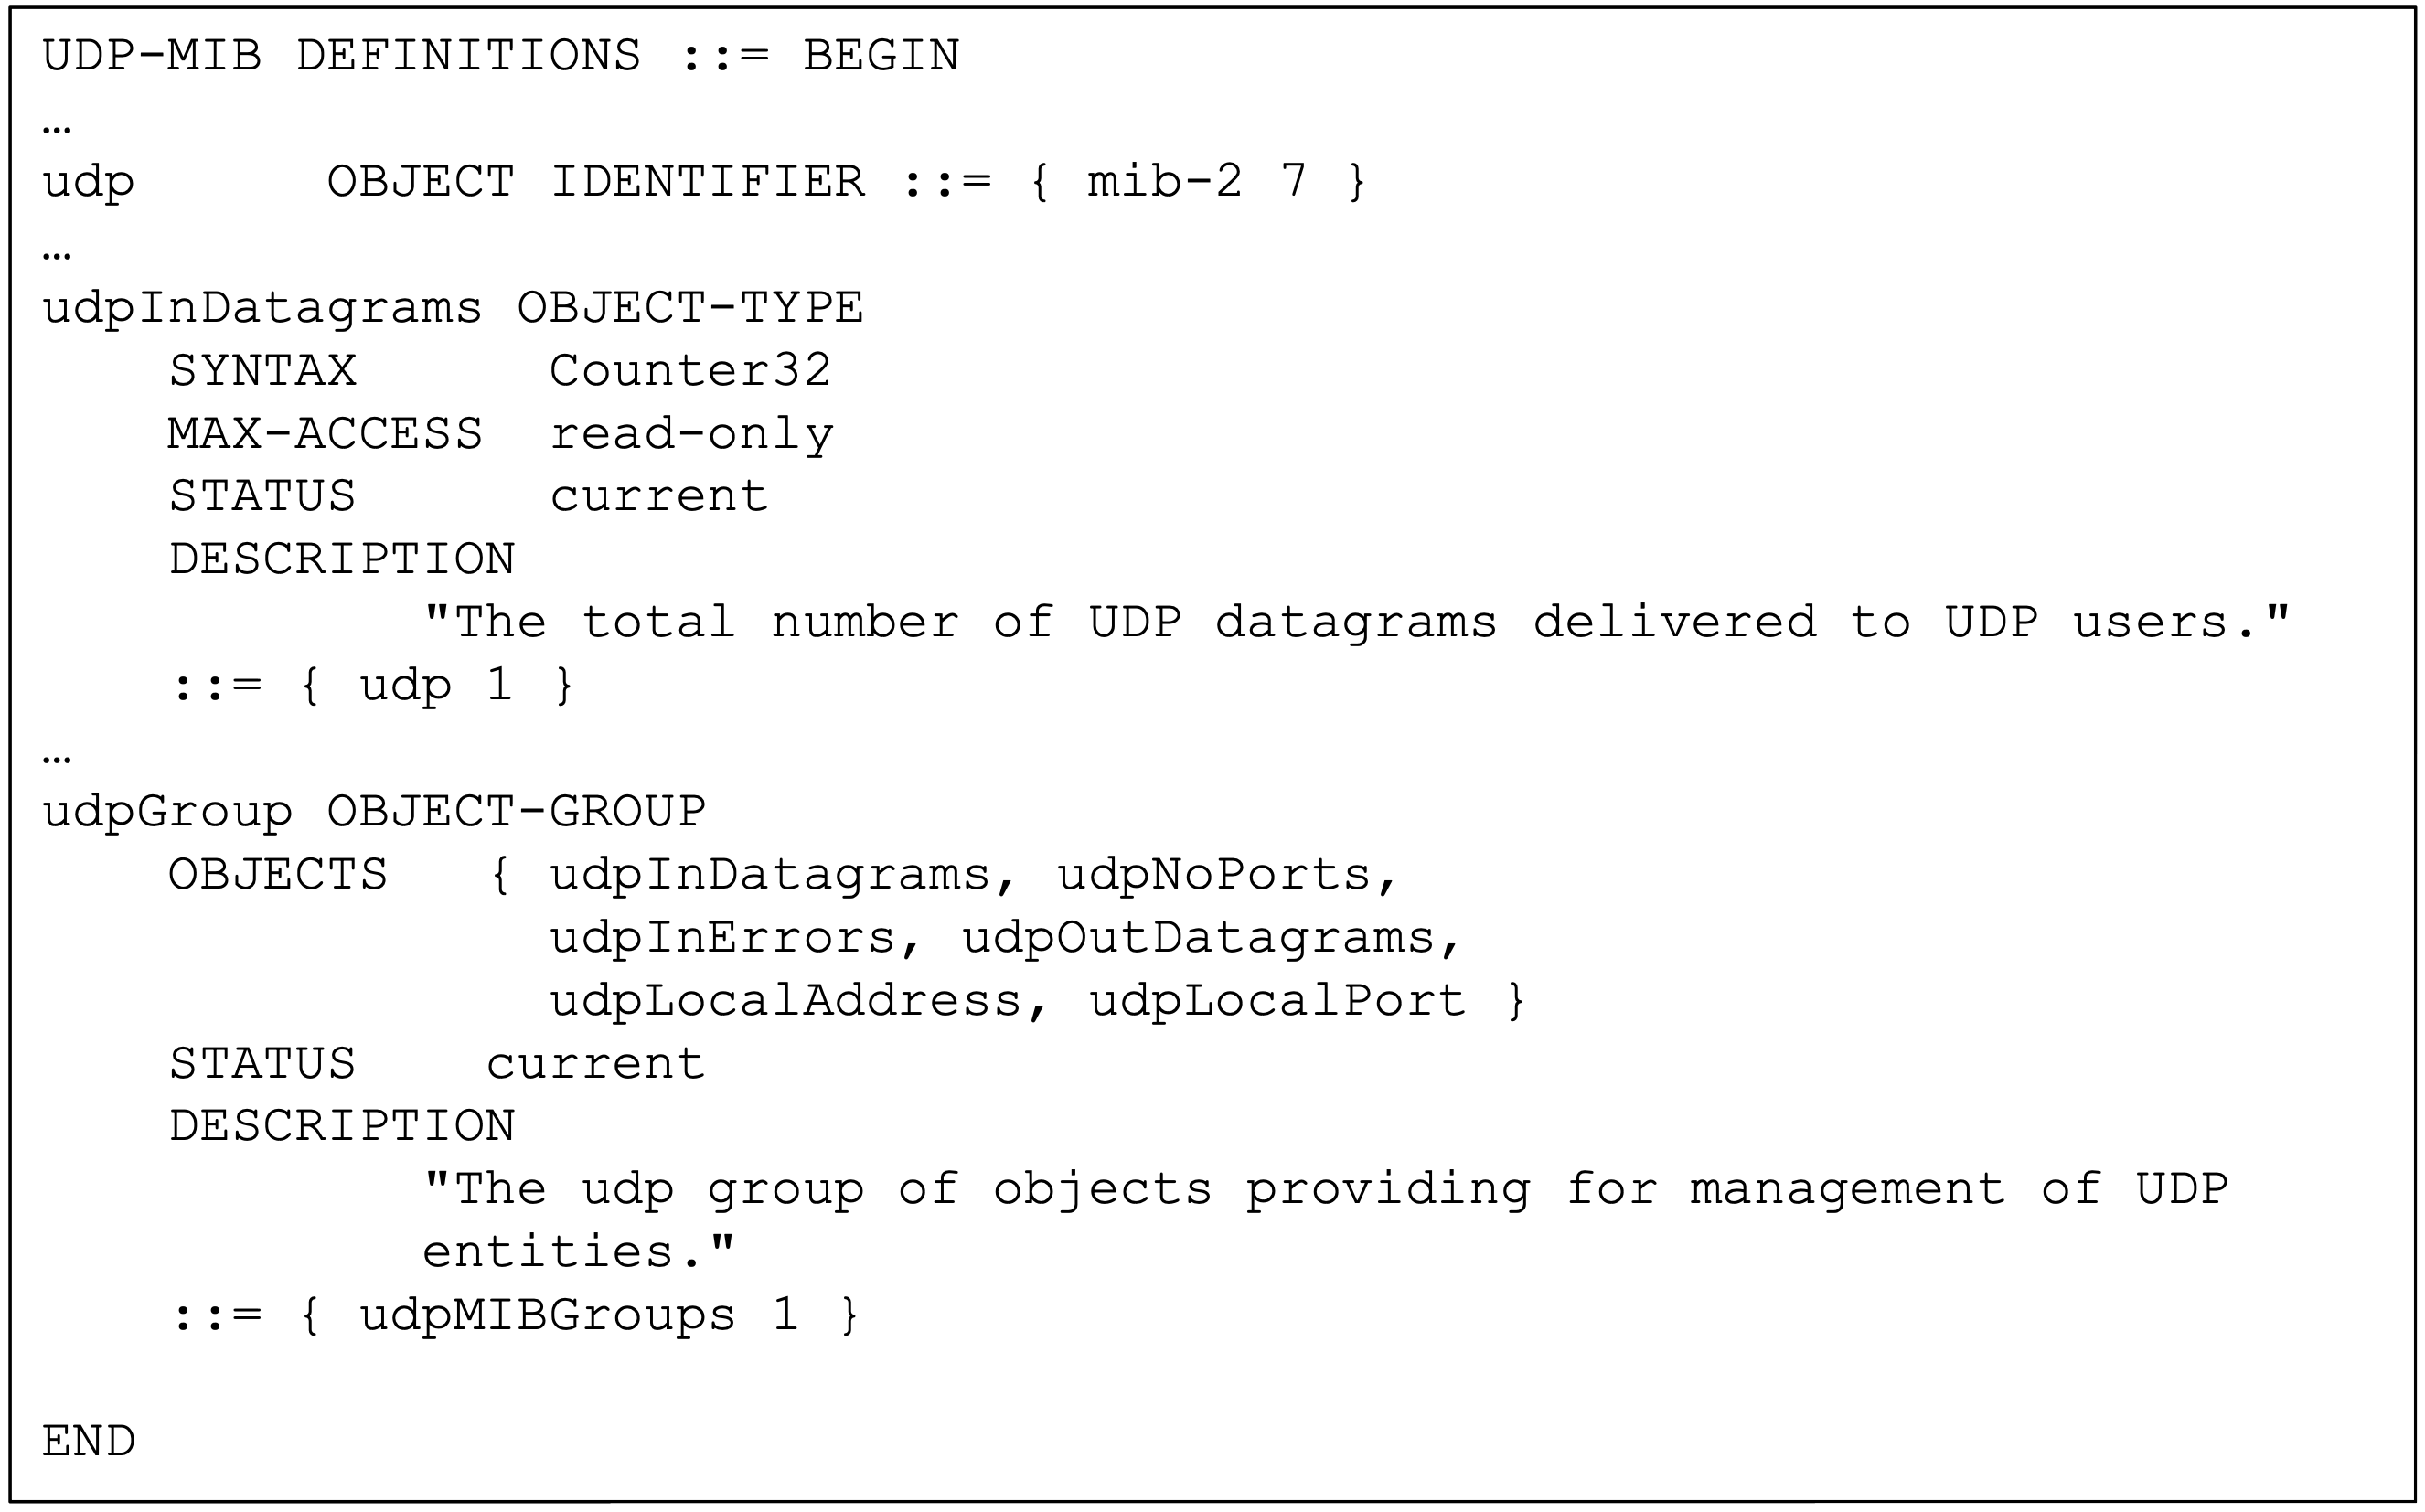
\includegraphics[scale=0.25]{MIB.png}
				\captionof{figure}{MIB-Modul}
			\end{center}
			\begin{center}
				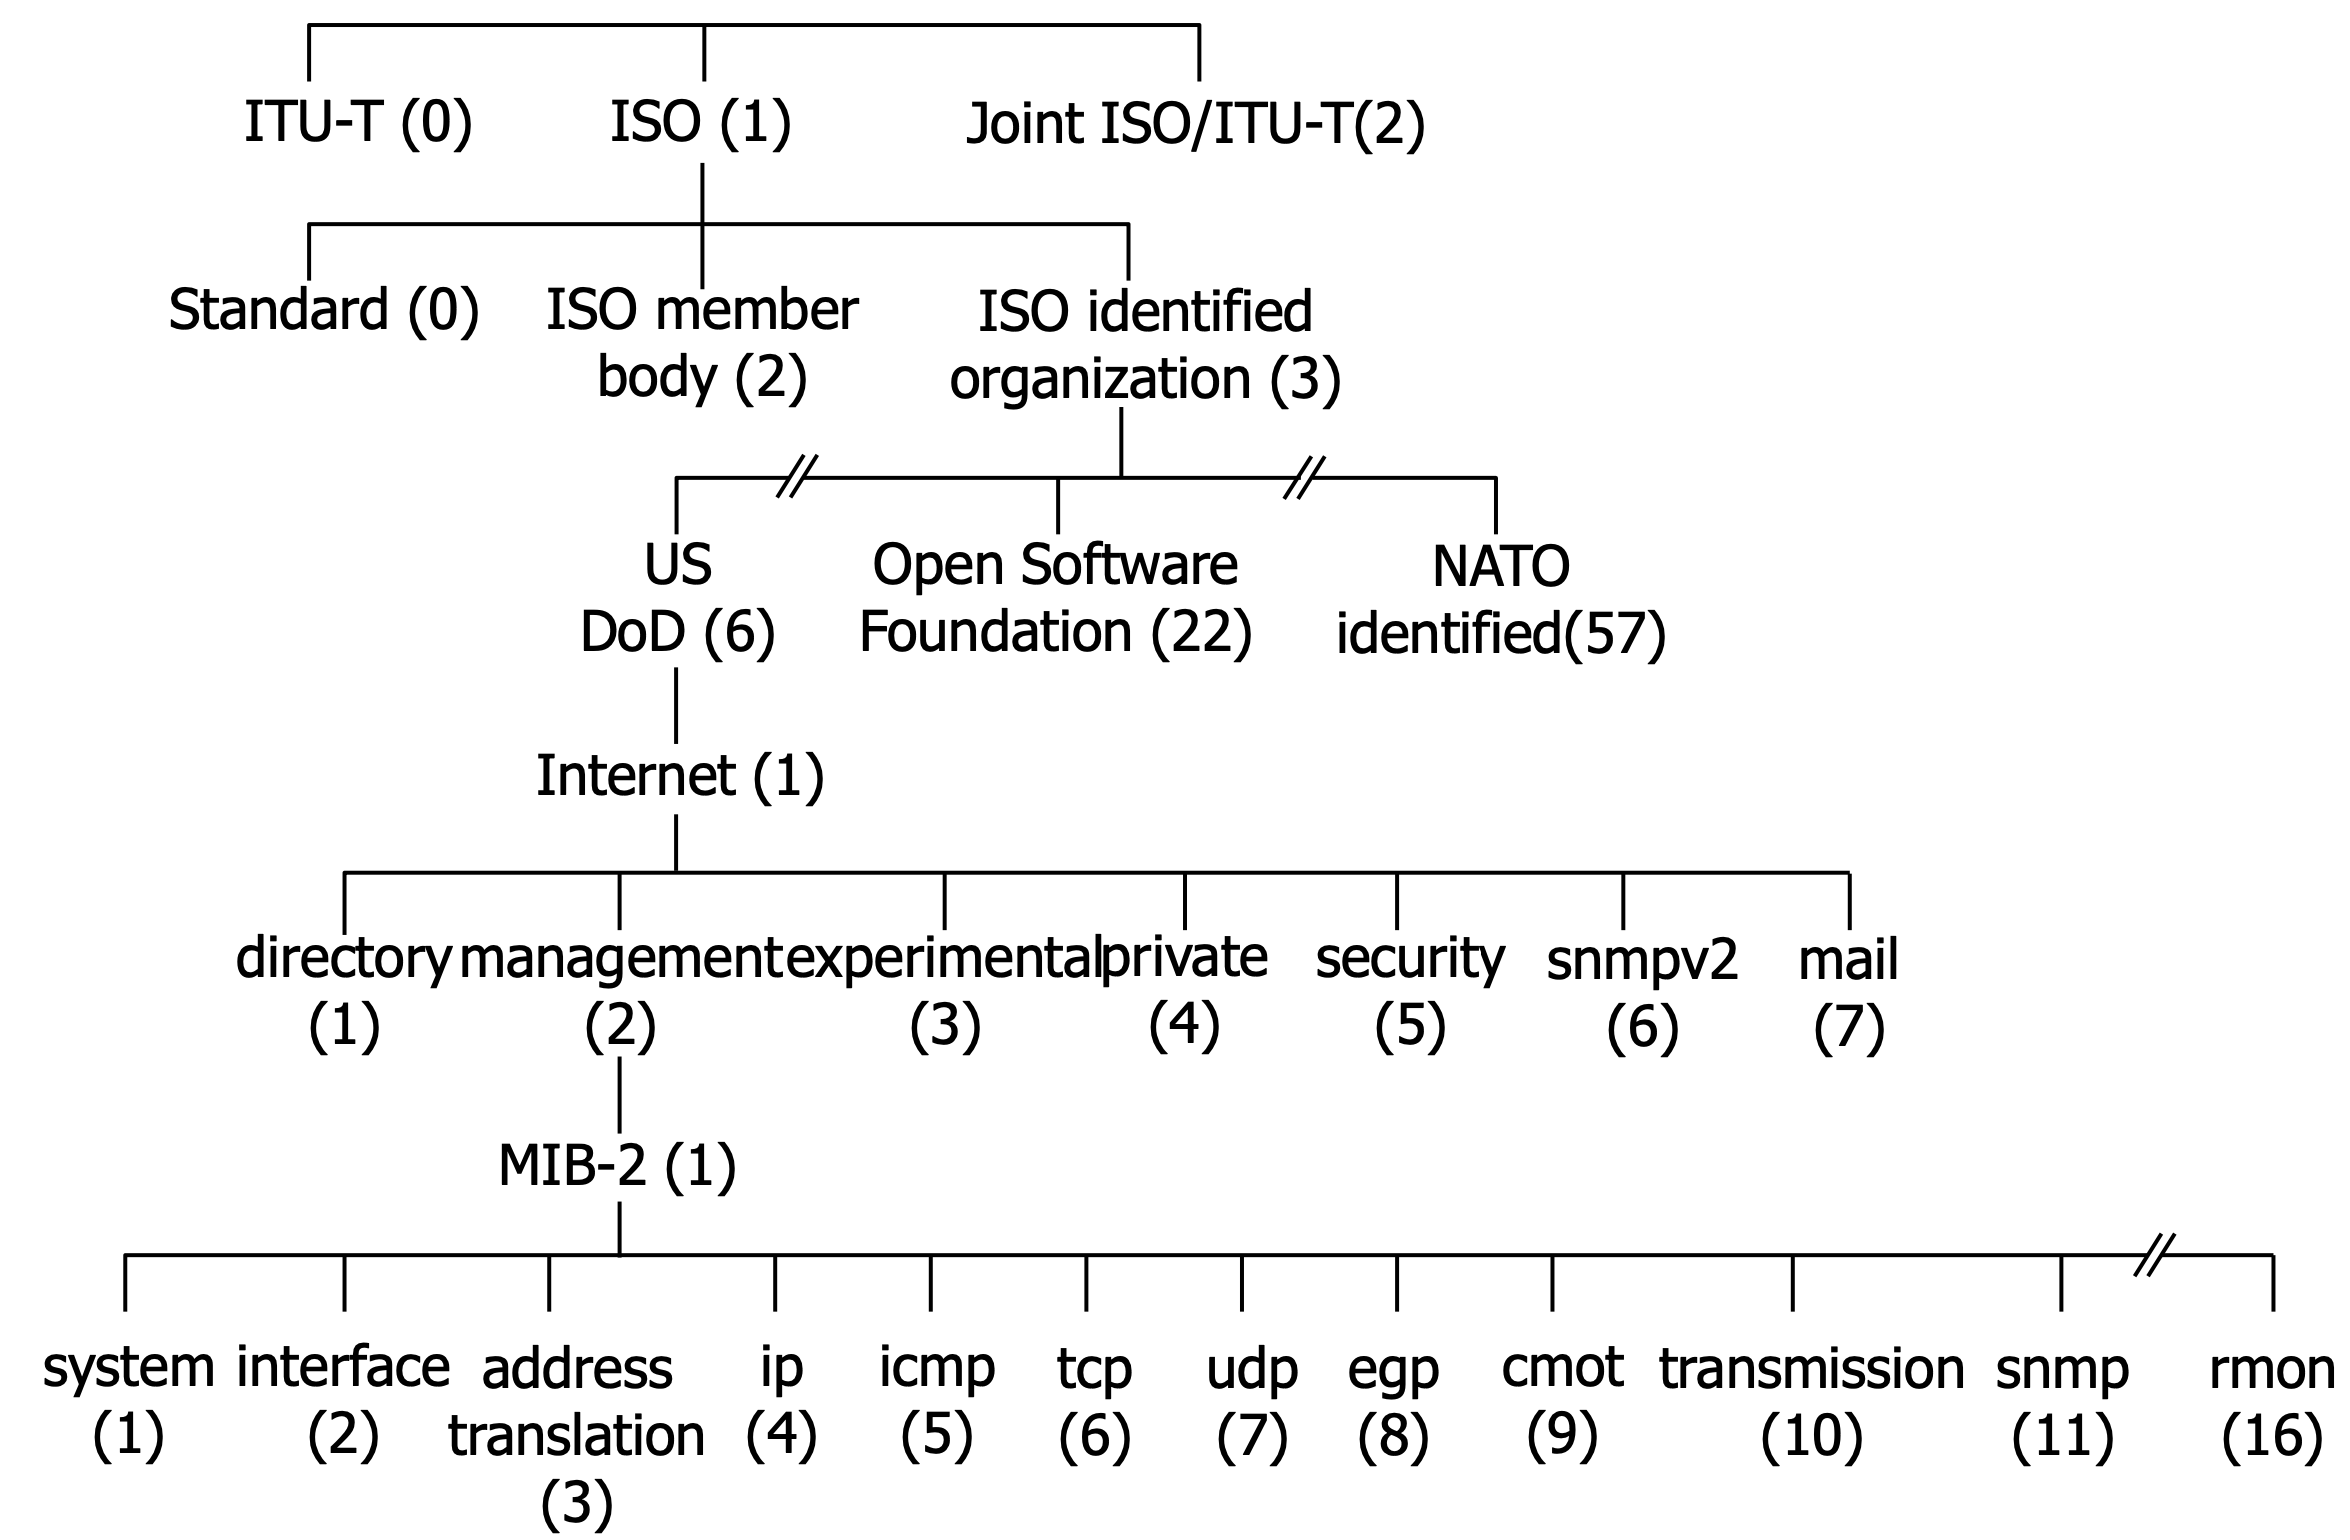
\includegraphics[scale=0.25]{OID.png}
				\captionof{figure}{OID}
			\end{center}
	\subsection{Domain Name Service (DNS)}
		DNS bildet Domain-Name auf Werte ab und ist als verteilte Datenbank, bestehend aus vielen Name-Servern, repräsentiert
		\subsubsection{Domain-Struktur}
			DNS implementiert hierarchischen Namensraum für Internet-Objekte
		\subsubsection{Hierachie von Name-Servern}
			\begin{itemize}
				\item \textbf{Root Name Server}: weltweit
				\item \textbf{Top-level Domain-Server} für com, org, net, ...
				\item ...
				\item \textbf{autoritativer Name-Server}: unterste Ebene für einzelne Organisationen
			\end{itemize}
		\subsubsection{Ressource Records}
			\begin{itemize}
				\item \textbf{TTL}: Time to Live, Dauer der Gültigkeit
				\item \textbf{Typ = A}:
					\begin{itemize}
						\item Wert = IPv4-Adresse
						\item AAAA-Einträge für IPv6-Adressen
					\end{itemize}
				\item \textbf{Type = NS}:
					\begin{itemize}
						\item Wert = Domainname eines Hosts, auf dem ein Server läuft, der Namen in der Domain auflösen kann
					\end{itemize}
				\item \textbf{Type = CNAME}: (Canonical Name)
					\begin{itemize}
						\item Wert = kanonischer Name eines Hosts, ermöglicht Aliasnamen
					\end{itemize}
				\item \textbf{Type = MX}: (Mail Exchange)
					\begin{itemize}
						\item Wert = Domain-Name des Hosts, auf dem der Mail-Server läuft
					\end{itemize}
			\end{itemize}
		\subsubsection{DNS-Protokoll}
			\begin{center}
				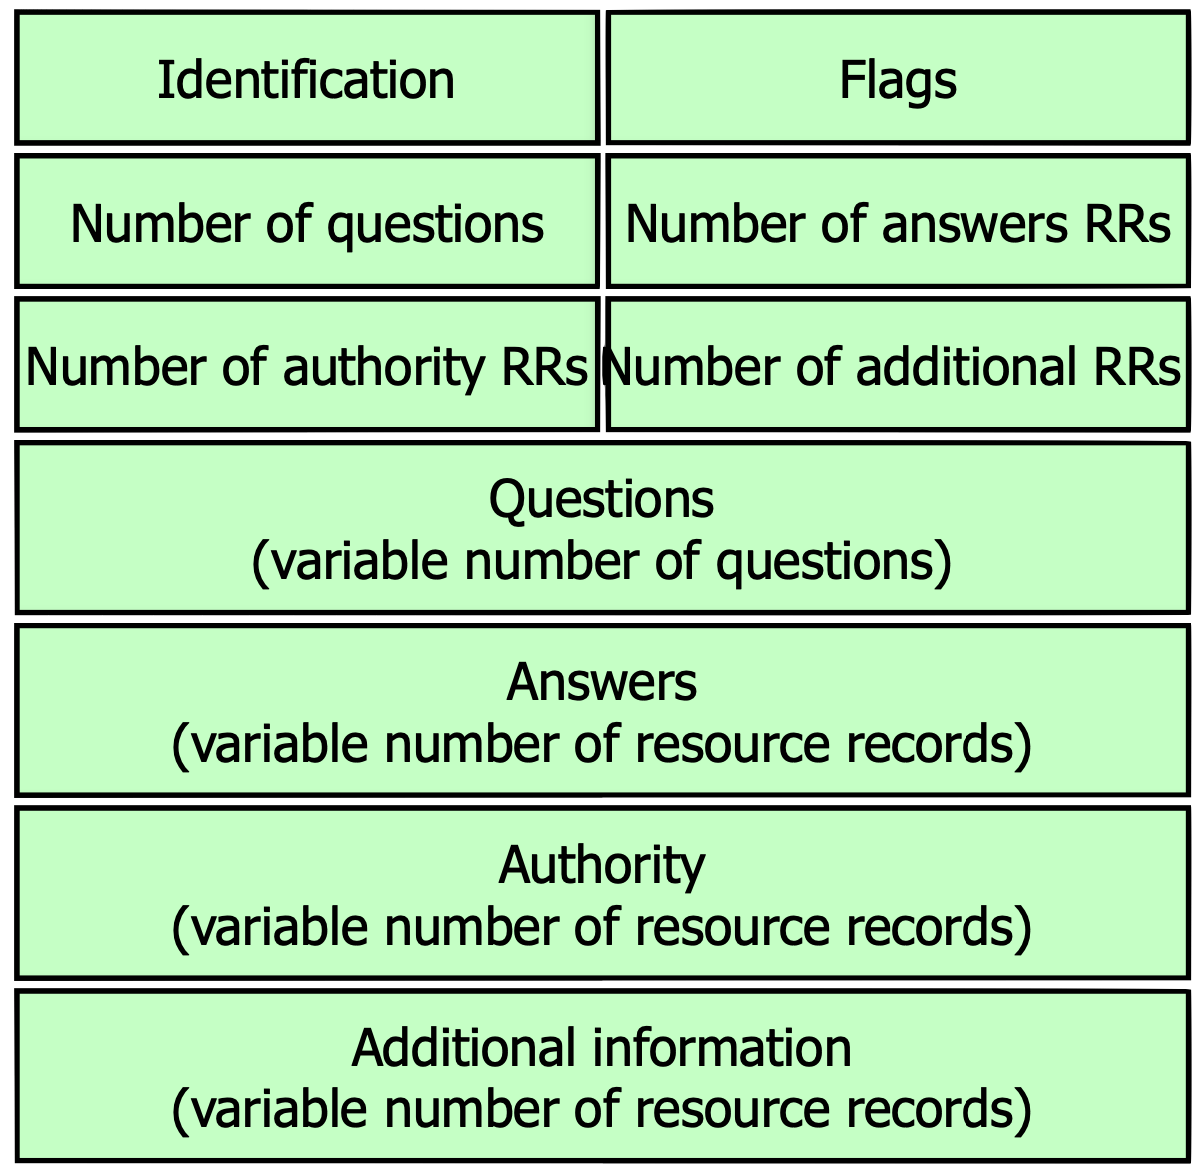
\includegraphics[scale=0.25]{DNS_Protokoll.png}
				\captionof{figure}{DNS Protokoll}
			\end{center}
		\subsubsection{Anfragen}
			iterativ:
			\begin{itemize}
				\item Antwort: anderer Server, der Name evtl. auflösen kann (oder keine Antwort)
				\item NS- und A-Datensatz
				\item Antwort wird sofort geliefert, es muss keine Information gespeichert werden, gut für hochfrequente Server
			\end{itemize}
			rekursiv:
			\begin{itemize}
				\item Antwort: Auflösung des Namens, die u.A. von anderen Servern geholt wird
				\item A-Datensatz
				\item bei Anfragen an einen anderen Server muss die Information gespeichert werden
			\end{itemize}
	\subsection{Content Distribution Network}
		Ziel: massive gleichzeitige Nutzung einer Webseite mit mehreren Mbit/s pro User zu realisieren \newline \newline
		Idee: sehr viele Spiegelserver geographisch verteilen und näher am Nutzer platzieren
		\subsubsection{Verteilung der Anfragen}
			\begin{itemize}
				\item \textbf{Server-basierte HTTP Redirection}: Server liefert aufgrund der IP-Adresse des Clients einen geeigneten anderen Server, erfordert zusätzliche RTT, Server-Betreiber muss Verteilung des Inhalts kennen, nicht bewährt
				\item \textbf{Client-nahe HTTP Redirection}: z.B. durch Web-Proxy, nicht bewährt
				\item \textbf{URL Rewriting}: Server liefert Basisseite, die URLs der eingebetteten Objekte werden umgeschrieben, mit dem Domain-Namen eines geeigneten Servers
				\item \textbf{DNS-basierte Redirection}: DNS-Server bilden Domain-Namen des Services auf Domain-Namen und zuletzt auf die IP-Adresse eines geeigneten Servers ab
			\end{itemize}

	\subsection{Socket-Programmierung}
		\subsubsection{Socket-Schnittstelle}
			\begin{itemize}
				\item verbreitetes API für Transportdienste
				\item Festlegung von TCP/UDP, IP-Adressen, Portnummern
			\end{itemize}
			\begin{center}
				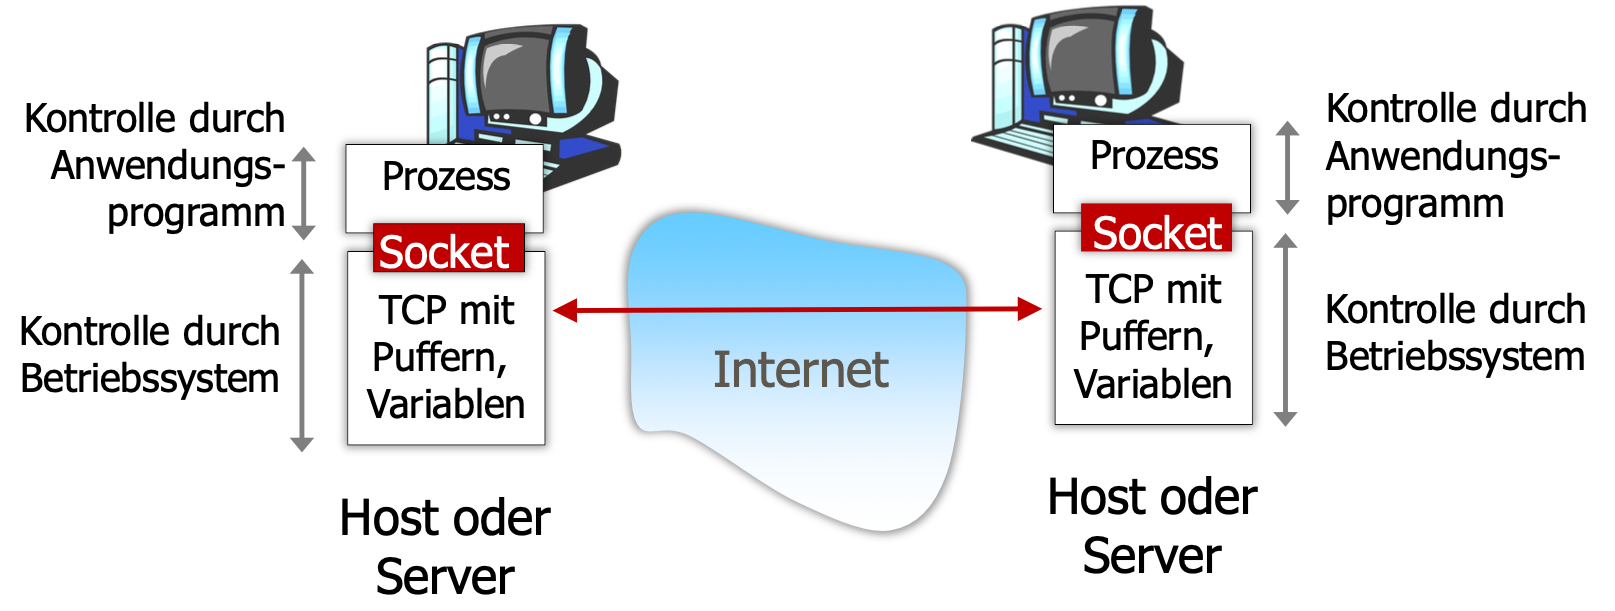
\includegraphics[scale=0.2]{Socket.png}
				\captionof{figure}{Socket}
			\end{center}
	\subsection{Peer-to-Peer}
		\textbf{Grundidee}: Inhalte nicht nur von zentralem Server, sondern auch von anderen Peers. Upload-Bitrate der Peers wird mitgenutzt
		\subsubsection{Unstrukturiert}
			\textbf{Zentralisiertes Verzeichnis}:
			\begin{itemize}
				\item Eintritt eines Peers: informiert zentralen Server über seine IP-Adresse und seine Inhalte
				\item Suche nach Inhalt: über zentralen Server
				\item Dateiübertragung: direkt zwischen Peers
				\item zentraler Server: juristischer und leistungstechnischer Schwachpunkt
			\end{itemize}
			\textbf{Dezentralität durch Fluten von Anfragen}
			\begin{itemize}
				\item Peers bilden Overlay-Netzwerk über TCP-Verbindungen
				\item anfragender Peer sendet Anfrage an alle seine Nachbarn im Overlay-Netzwerk
				\item diese vergleichen Anfragen mit den von ihnen angebotenen Inhalten
				\item wenn nicht gefunden werden die Anfragen an mehrere Nachbarn weitergeleitet
				\item das Fluten wird durch einen maximalen Hopcount begrenzt
				\item bei fund wird dem anfragendem Peer geantwortet (nicht dem ursprünglichen, womit seine Identität geheim bleibt)
				\item Verbindung wird mittels HTTP zwischen Quelle und Ursprung hergestellt
			\end{itemize}
			\textbf{Hybrid} \newline \newline
				Peers bilden Gruppen, einer ist Group-Leader, P2P-Netzwerke in Gruppen und zwischen Leadern $\Rarr$ besser skalierbar
		\subsubsection{Strukturiert}
			\textbf{Verteilte Hash-Tabllen}
			\begin{itemize}
  				\item Peers bilden ringförmiges Overlay-Netz
  				\item jedem Peer wird ein zufälliger Bezeichner $p(0\leq p\leq 2^m-1)$ aus ringförmigen Bezeichnerraum mit m Bits zugewiesen
  				\item jedem Datenelement wird mittels Hash-Funktion ein Schlüssel k ebenfalls aus diesem Raum zugewiesen
  				\item Nachfolger von k:
  					\begin{itemize}
  						\item Datenelement mit Schlüssel k wird auf Nachfolger p von k gespeichert (Nachfolger darf Knoten k selbst sein)
  						\item der nächste Peer im Ring, formal: Peer p mit dem kleinsten $a\geq0$, sodass $p=\texttt{succ}(k)=(k+a)\mod2^m$ existiert
  						\item auslesen eines Datenelements mit Schlüssel k erfolgt auf Peer succ(k)
					\end{itemize}
			\end{itemize}
		\subsubsection{Bittorrent}
			\begin{itemize}
				\item \textbf{Torrent}: Schwarm von Peers fu2r gleiche Datei
				\item \textbf{Chunks}: Teile der zu verteilenden Datei
				\item \textbf{Tracker}: Server, bei dem sich Peers registrieren
				\item .torret-Datei mit Metadaten über zu verbelibende Datei und Tracker
				\item neuer Peer tritt Schwarm bei:
					\begin{itemize}
						 \item A registriert sich bei Tracker und erhält IP-Adressen zufälliger anderer Peers des Schwarms
						 \item A baut TCP-Verbindung zu einigen dieser Peers auf, fragt Liste der Chunks in ihrem Besitz nach und sendet Anfragen für Chunks
						 \item Rarest First: A fragt die seltensten Chunks der Peers zuerst nach, dadurch gleichmäßige Verteilung
						 \item Incentive Mechanismus (Tit-for-Tat): A misst Antwortrate der Peers und antwortet an diese in entsprechendem Anteil der Upload-Rate
						 \item neue Nachbarn werden zufällig dazu genommen
					\end{itemize}
			\end{itemize}
		\subsubsection{Bitcoin}
			\begin{itemize}
				\item \textbf{Allgemein}
					\begin{itemize}
						\item Transaktionen an öffentliche Bitcoin-Adressen, digital signiert mit privatem Schlüssel, Versendung in unstrukturiertem P2P-Netzwerk
						\item Miner sammeln Transaktionen in Blöcken und führen Proof-of-Work durch
						\item Incentive bei erfolgreichem Schürfen eines Blocks
						\item Blockchain ist verteilte Datenbank, auch distributed Ledger genannt, mit allen Transaktionen seit Beginn und erlaubt die Vermeidung von Double-Spending 
					\end{itemize}
				\item \textbf{Adressen}
					\begin{itemize}
						\item abgeleitet aus privaten und öffentlichen Schlüsseln, basierend auf elliptischen Kurven
						\item Private Key: (256 Bits, hexa)
						\item Public Key: (256 Bits, hexa), aus Private Key berechnet
						\item Adresse: SHA-256 2x auf Public Key anwenden und mit Base58 (Alphabeth) kodieren
						\item Wallet: Verwaltet die Schlüssel, welche aus einem Seed abgeleitet wurden
					\end{itemize}
				\item \textbf{Transaktionen}	
					\begin{itemize}
						\item Unspent Transaction Outputs (UTXO) werden zu andern Adressen transferiert
						\item Input: UTXO + Unlocking-Script (privater Schlüssel, der Adresse)
						\item Output: Transfer zu neuer Bitcoin-Adresse + Locking-Script (z.B. Adresse)
						\item Fluten: An Peers versenden, diese verifizieren Transaktionen, überprüfen auf Double-Spending in Blockchain und senden weiter
					\end{itemize}
				\item \textbf{Blockchain}
					\begin{itemize}
						\item Miner erstellt Blöcke mit Transaktionen (1 MB)
						\item Block-Header (80 Bytes)
						\item Proof-of-Work: Berechnung von Hash (SHA-256) kleiner als Difficulty (führende Zahl von Nullen) Lösung durch ausprobieren
						\item Wenn Block gefunden: Fluten, Peers verifizieren den Block und berechnen bei Akzeptanz nächsten Block, dadurch wächst die Blockchain im Mittel alle 10 min
						\item ergibt ca. 7 Transaktionen pro Sekunde
					\end{itemize}
			\end{itemize}

				





			
			
			
